%*****************************************
\chapter{Fundamental Skills}\label{ch01:fundamentals}
%*****************************************
% Second pass corrections made and grammar checked 220622

Microsoft\textsuperscript{\textregistered} Excel\textsuperscript{\textregistered} is a tool that can be used in virtually all careers and is valuable in professional and personal settings. Applications as diverse as keeping track of medications in inventory for a hospital or creating a financial retirement plan can be made efficiently and accurately with Excel. This chapter introduces the fundamental skills necessary to start with Excel. Most people find that learning only a few skills makes them very productive in a short time. 

\section{Overview of Microsoft Excel}

\begin{center}
	\begin{objbox}{Learning Objectives}
		\begin{itemize}
			\setlength{\itemsep}{0pt}
			\setlength{\parskip}{0pt}
			\setlength{\parsep}{0pt}
			
			\item Examine the value of using Excel to make decisions.
			\item Learn how to start Excel.
			\item Become familiar with the Excel workbook.
			\item Understand how to navigate worksheets.
			\item Examine the Excel Ribbon.
			\item Examine the right-click menu options.
			\item Learn how to save workbooks.
			\item Examine the Status Bar.
			\item Become familiar with the features in the Excel Help window.
			
		\end{itemize}
	\end{objbox}
\end{center}

Microsoft\textsuperscript{\textregistered} Office\textsuperscript{\textregistered} contains various tools to help people accomplish personal and professional objectives. However, Excel is perhaps the most versatile and widely used of all Office applications. Most career paths use Excel to accomplish professional objectives, often daily. This chapter provides an overview of the Excel application and an orientation for accessing the commands and features of an Excel workbook.

\subsection{Making Decisions With Excel}

Taking a superficial view, Excel is a tool for entering quantitative data into an electronic spreadsheet to apply one or several mathematical computations. These computations ultimately convert that quantitative data into information. The information produced in Excel can be used to make decisions in both professional and personal contexts. For example, Excel can help retailers determine how much inventory to stock or balance income with outgo. Concerning personal decisions, Excel can help determine how much money is available to spend on a house, car payment, or savings for retirement. This text demonstrates using Excel to make these decisions and many more.

Figure \ref{01:fig01} shows a completed Excel worksheet that will be constructed in this chapter. The information shown in this worksheet is the top-line sales data for a hypothetical merchandise retail company. The worksheet data can help this retailer determine how many salespeople are needed each month, how much inventory is needed to satisfy sales, and what types of products should be purchased.

\begin{figure}[H]
	\centering
	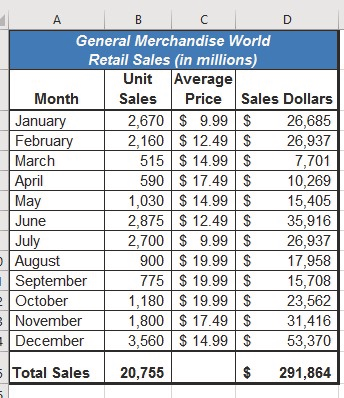
\includegraphics[width=\maxwidth{.95\linewidth}]{gfx/ch01_fig01}
	\caption{Example of an Excel Worksheet}
	\label{01:fig01}
\end{figure}

\subsection{Starting Excel}

\begin{enumbox}
	\begin{enumerate}
		\item Locate Excel on the Windows menu.
		\item Click \fmtButton{Microsoft Excel} to launch the Excel application.
		\item Click the first option, \fmtButton{Blank Workbook}.
	\end{enumerate}
\end{enumbox}

\subsection{The Excel Workbook}

Once Excel is started, a blank workbook will open. A workbook is an Excel file containing one or more worksheets (sometimes called spreadsheets). Figure \ref{01:fig02} shows a blank workbook after starting Excel. Take some time to become familiar with this screen. (\textit{Note: the worksheet screen may be slightly different depending on the Excel version.})

\begin{figure}[H]
	\centering
	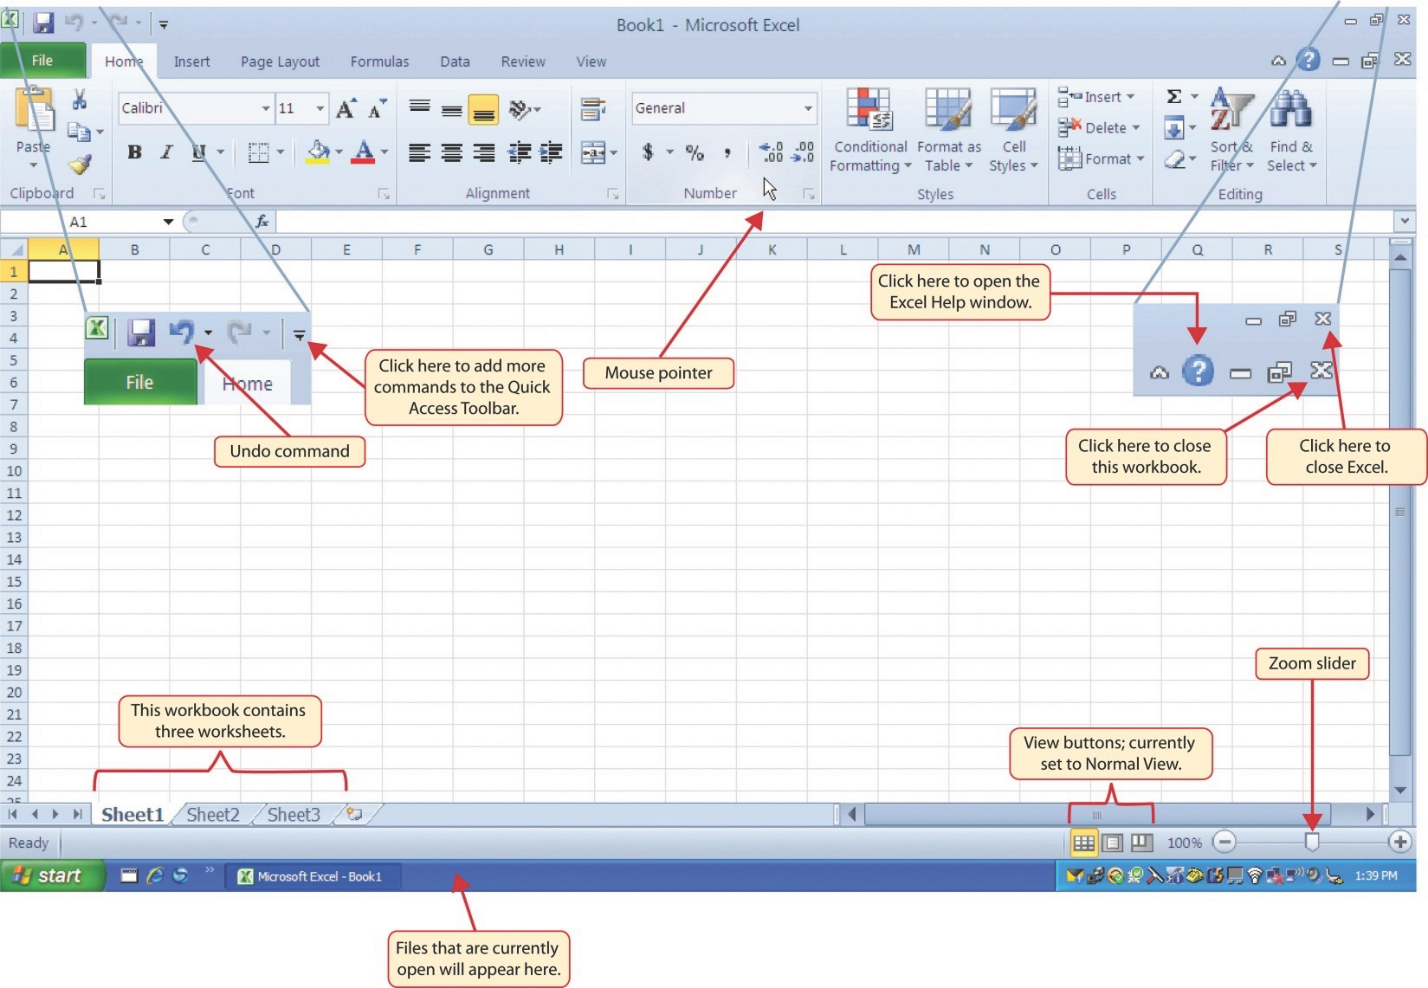
\includegraphics[width=\maxwidth{.95\linewidth}]{gfx/ch01_fig02}
	\caption{Blank Workbook}
	\label{01:fig02}
\end{figure}

The workbook should already be maximized (or shown at full size) once Excel is started, as shown in Figure \ref{01:fig02}. However, if the screen looks like Figure \ref{01:fig03} after starting Excel, click the \textit{Maximize} button, as shown in the figure.

\begin{figure}[H]
	\centering
	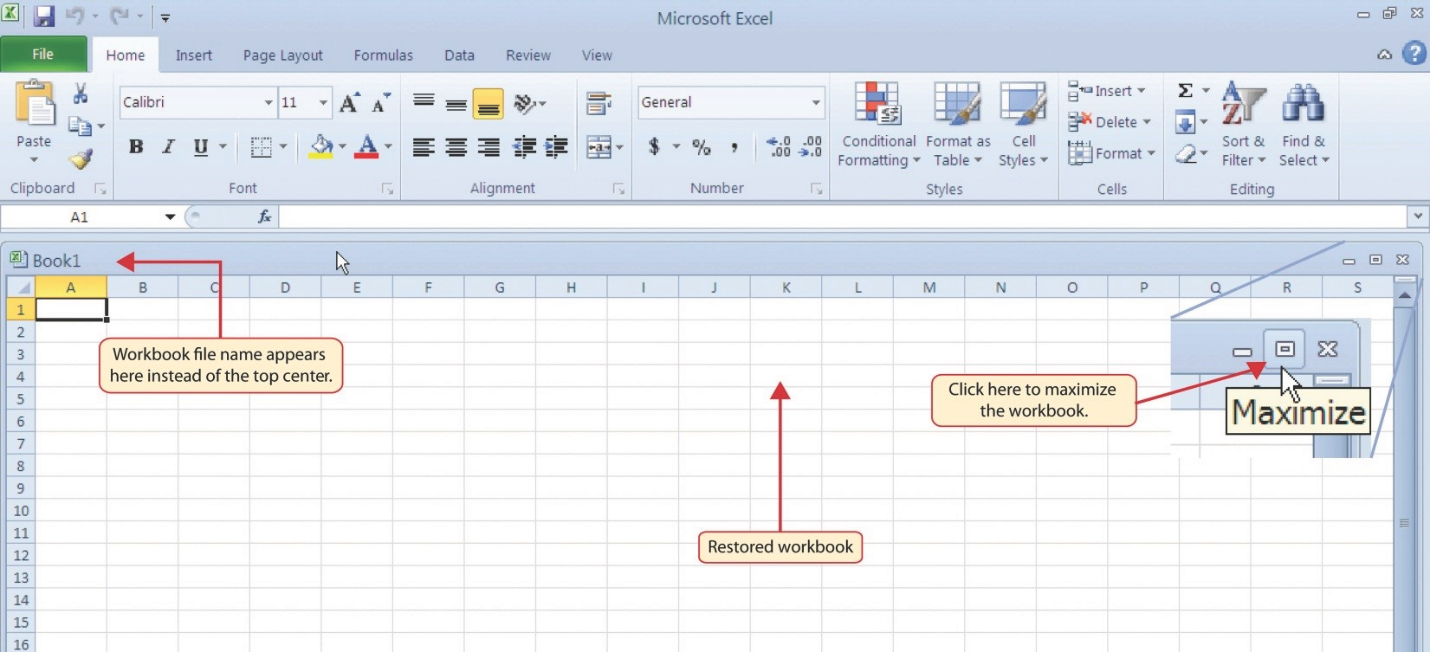
\includegraphics[width=\maxwidth{.95\linewidth}]{gfx/ch01_fig03}
	\caption{Restored Workbook}
	\label{01:fig03}
\end{figure}

\subsection{Navigating Worksheets}

Data is entered and managed in an Excel worksheet. The worksheet contains several rectangles called cells for entering numeric and non-numeric data. Each cell in an Excel worksheet is located at an address defined by a column letter followed by a row number. For example, the cell currently activated in Figure \ref{01:fig03} is $ A1 $. This location would be called cell location $ A1 $ or cell reference $ A1 $. The following steps explain how to navigate an Excel worksheet.

\begin{itemize}
	\item Place the mouse pointer over cell \fmtLoc{D5} and left-click.
	\item Check to ensure \fmtLoc{Column D} and \fmtLoc{Row 5} are selected, as shown in Figure \ref{01:fig04}.
\end{itemize}

\begin{figure}[H]
	\centering
	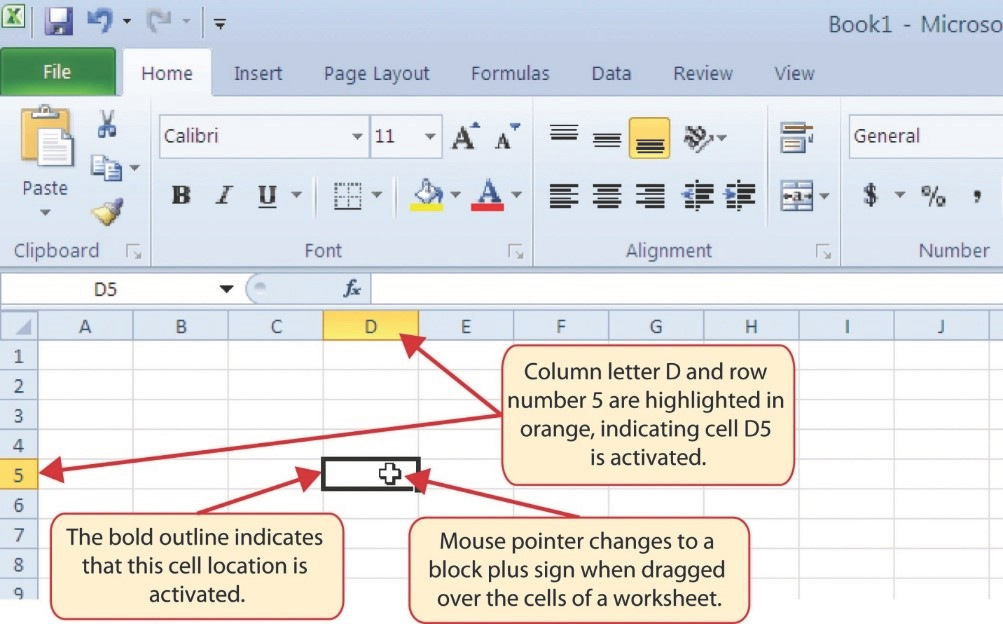
\includegraphics[width=\maxwidth{.95\linewidth}]{gfx/ch01_fig04}
	\caption{Activating a Cell Location}
	\label{01:fig04}
\end{figure}

The following steps explain selecting a range of cells in an Excel worksheet.

\begin{enumbox}
	\begin{enumerate}
		\item Click the mouse pointer in cell \fmtLoc{A1}.
		\item Click and hold the left mouse button and drag the mouse pointer to cell \fmtLoc{D5}.
		\item Release the left mouse button. Several cells are now selected, as shown in Figure \ref{01:fig05}.
	\end{enumerate}
\end{enumbox}

\begin{figure}[H]
	\centering
	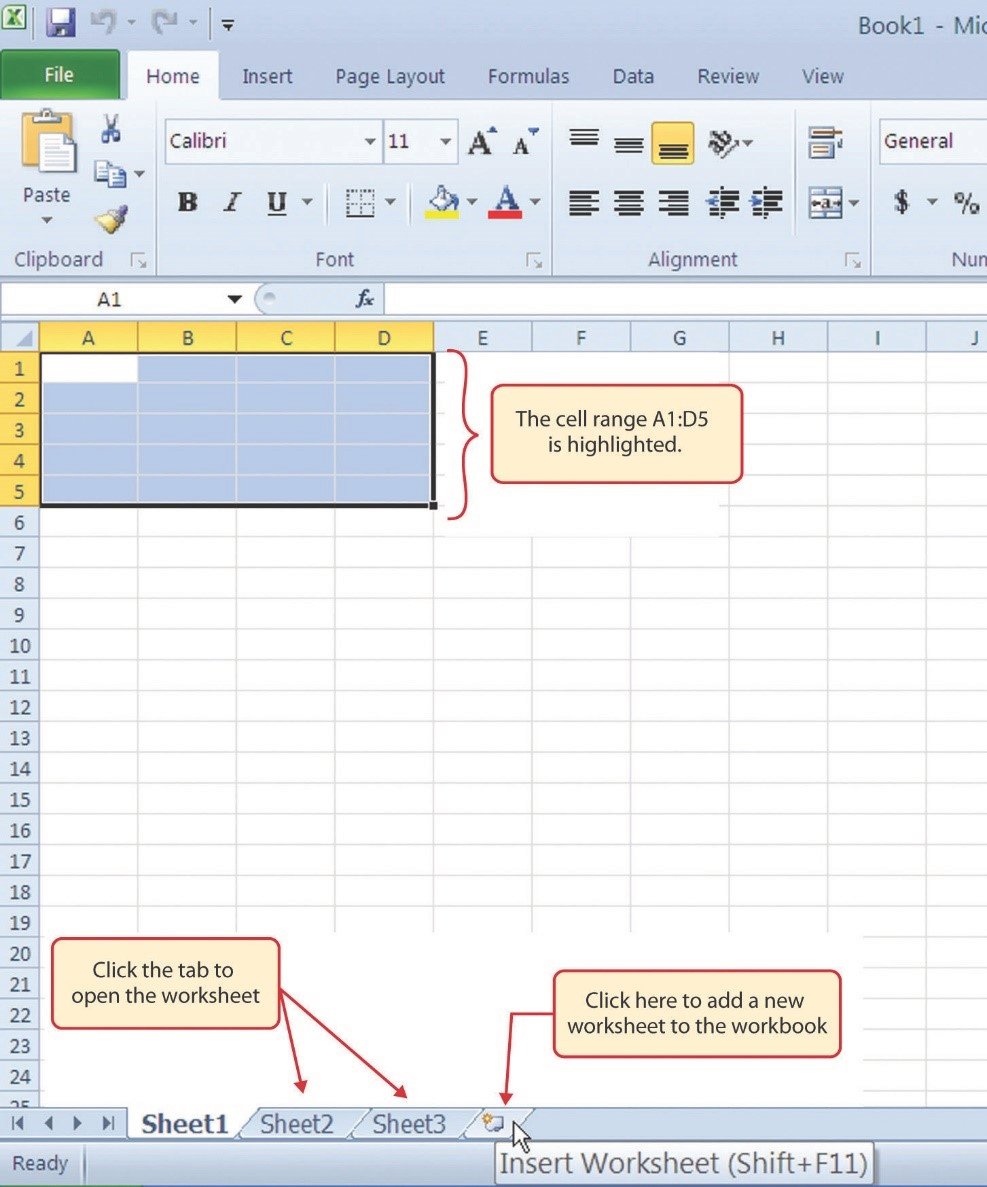
\includegraphics[width=\maxwidth{.95\linewidth}]{gfx/ch01_fig05}
	\caption{Selecting a Range of Cells}
	\label{01:fig05}
\end{figure}

Multiple selected cells are called a cell range and are usually annotated as $ A1 $:$ D5 $. The first cell in the range is in the top left corner, and the second cell is in the lower right corner.

\begin{enumbox}
	\begin{enumerate}
		\item At the bottom of the screen are tabs that identify different worksheets. Depending on the Excel version being used, one tab or several may be displayed, as shown in Figure \ref{01:fig05}. If there is only one sheet, clicking \fmtButton{Insert Worksheet} adds a new worksheet. Different versions of Excel use \fmtButton{$ + $} or \fmtButton{Insert Worksheet} buttons. For this exercise, add worksheets as necessary, so three are available.
		\item Click the \fmtWorksheet{Sheet1} tab at the bottom of the screen to activate it, as shown in Figure \ref{01:fig05}.
	\end{enumerate}
\end{enumbox}

\begin{center}
	\begin{shtcutbox}{Keyboard Shortcuts}
		\textbf{Basic Worksheet Navigation}
		\\
		\begin{itemize}
			\setlength{\itemsep}{0pt}
			\setlength{\parskip}{0pt}
			\setlength{\parsep}{0pt}

			\item Use the arrow keys on the keyboard to move the cell pointer to different cells on the worksheet.
			\item Press and hold \fmtKeystroke{Shift}, then tap the arrow keys on the keyboard to select a range of cells in a worksheet.
			\item Press and hold \fmtKeystroke{Ctrl}, then tap \fmtKeystroke{Page Down} or \fmtKeystroke{Page Up} to open other worksheets in a workbook.

		\end{itemize}
	\end{shtcutbox}
\end{center}

\subsection{The Excel Ribbon}

Excel's features and commands are found in the \textit{Ribbon}, the upper area of the Excel screen that contains several tabs running across the top. Each tab provides access to a different set of Excel commands. Figure \ref{01:fig06} shows the commands available in the \textit{Home} tab of the Ribbon. Table \ref{01:tab01}, \textit{Command Overview for Each Tab of the Ribbon}, provides an overview of the commands found in each tab of the Ribbon.

\begin{figure}[H]
	\centering
	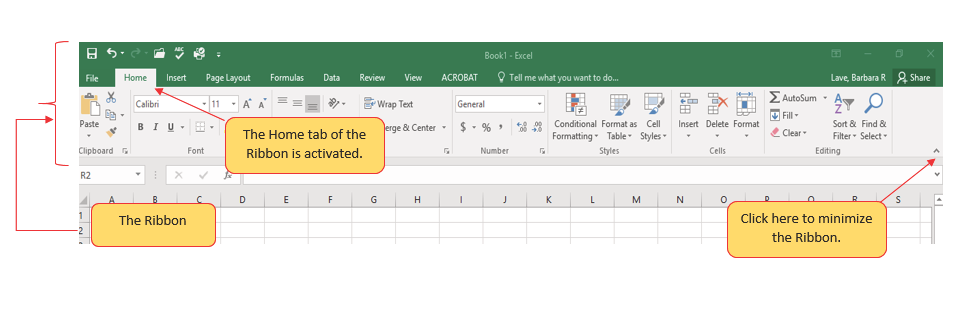
\includegraphics[width=\maxwidth{.95\linewidth}]{gfx/ch01_fig06}
	\caption{Home Tab of the Ribbon}
	\label{01:fig06}
\end{figure}

%The table is full of sentence fragments. Maybe that's OK, but I may want to rethink it.
\begin{table}[H]
	\rowcolors{1}{}{tablerow} % zebra striping background
	{\small
		%\fontsize{8}{10} \selectfont %Replace small for special font size
		\begin{longtable}{L{0.75in}L{3.50in}} %Left-aligned, Max width: 4.25in
			\textbf{Tab} & \textbf{Description} \endhead
			\hline

			File & Also known as the \textit{Backstage View} of the Excel workbook. It contains all commands for opening, closing, saving, and creating new Excel workbooks and includes print commands, document properties, e-mailing options, and help features. Excel's user options are also found in this tab.\\

			Home & The most frequently used formatting commands are found in this tab, along with commands for cutting, copying, pasting, and inserting and deleting rows and columns.\\
			
			Insert & Used to insert objects such as charts, pictures, shapes, PivotTables, Internet links, symbols, or text boxes.\\
			
			Page Layout & Commands used to prepare a worksheet for printing and show the grid lines on a worksheet are on this tab.\\
			
			Formulas & Includes commands for adding mathematical functions to a worksheet and tools for auditing mathematical formulas.\\
			
			Data & Used when working with external data sources such as Microsoft® Access®, text files, or the Internet. This tab also contains sorting commands and access to scenario tools.\\
			
			Review & Includes Spelling and Track Changes features. This tab also contains protection features for worksheets and workbooks.\\
			
			View & Used to adjust the visual appearance with tools like Zoom and Page Layout.\\

			\rowcolor{captionwhite}
			\caption{Command Overview for Ribbon Tabs}
			\label{01:tab01}
		\end{longtable}
	} % End small
\end{table}

The Ribbon shown in Figure \ref{01:fig06} is complete or maximized. Having a full Ribbon makes commands always visible while developing a worksheet. However, the Ribbon may take up too much space around the worksheet on a small screen. If this is the case, it can be minimized by clicking the button shown in Figure \ref{01:fig06}. When minimized, the Ribbon will show only the tabs and not the command buttons. Clicking a tab makes the command buttons appear until a command is selected or the mouse has clicked anywhere on the worksheet. Once the ribbon is expanded, it can be pinned open by clicking the \fmtButton{pin} button at its lower-left corner.

\begin{center}
	\begin{shtcutbox}{Keyboard Shortcuts}
		\textbf{Minimizing or Maximizing the Ribbon}
		\\
		\begin{itemize}
			\setlength{\itemsep}{0pt}
			\setlength{\parskip}{0pt}
			\setlength{\parsep}{0pt}
			
			\item Press and hold \fmtKeystroke{Ctrl}, then tap \fmtKeystroke{F1} to toggle between the maximized and minimized view of the ribbon.
			
		\end{itemize}
	\end{shtcutbox}
\end{center}

\subsection{Quick Access Toolbar and Right-Click Menu}

The \textit{Quick Access Toolbar} is on the upper left of the Excel screen above the Ribbon, as shown in Figure \ref{01:fig07}. This area provides access to the most frequently used commands, such as Save and Undo. The \textit{Quick Access Toolbar} can be customized by adding extensively used commands. Placing commands on the \textit{Quick Access Toolbar} makes it unnecessary to find them on the Ribbon. To customize the \textit{Quick Access Toolbar}, click the down arrow shown in Figure \ref{01:fig07}. Clicking the down arrow opens a menu of commonly used commands that can be added to the \textit{Quick Access Toolbar}. Select the \textit{More Commands} option if the desired command is not on the list to open a menu containing every command on the ribbon.

\begin{figure}[H]
	\centering
	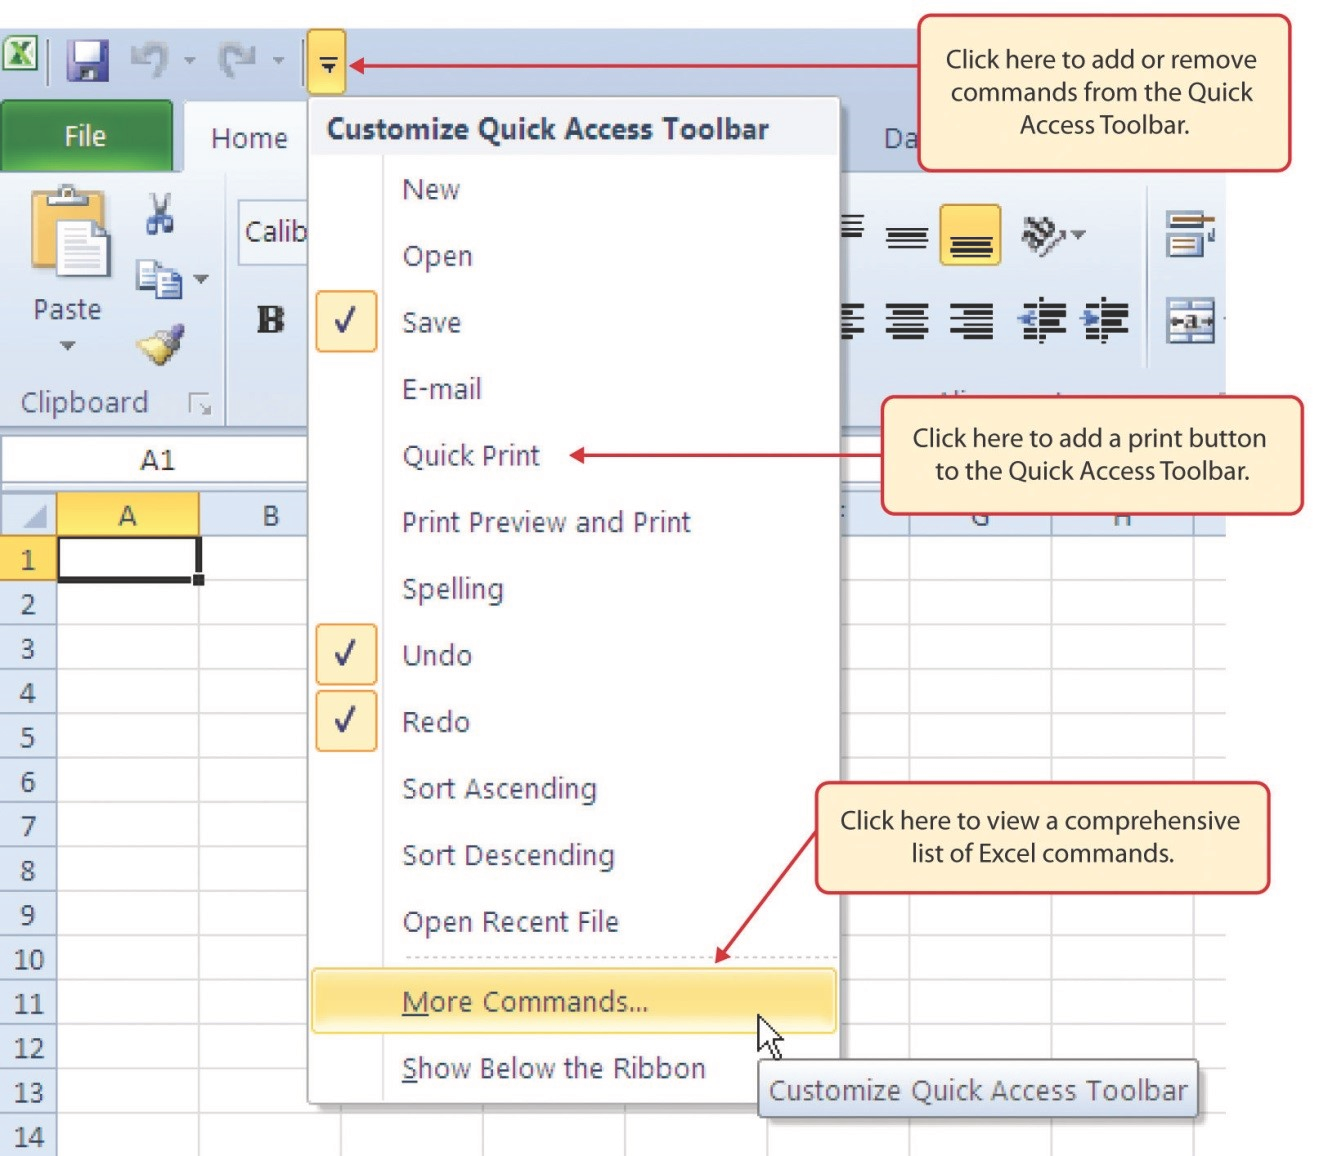
\includegraphics[width=\maxwidth{.95\linewidth}]{gfx/ch01_fig07}
	\caption{Customizing the Quick Access Toolbar}
	\label{01:fig07}
\end{figure}

Commands can also be accessed by right-clicking anywhere on the worksheet and selecting them from a context menu. \ref{01:fig08} shows an example of the commands available in the context menu.

\begin{figure}[H]
	\centering
	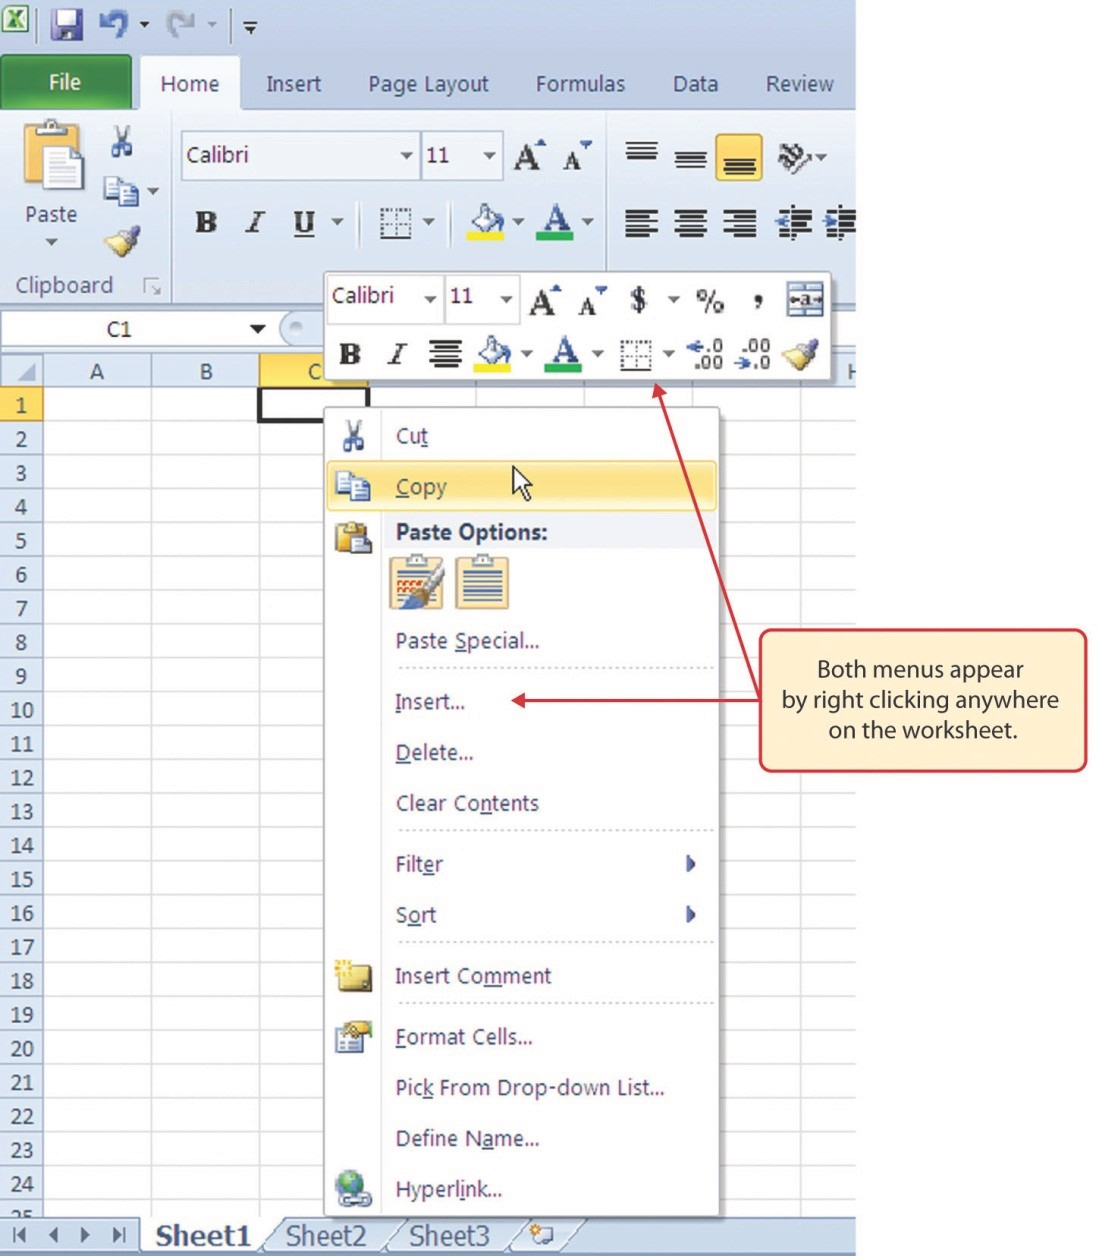
\includegraphics[width=\maxwidth{.95\linewidth}]{gfx/ch01_fig08}
	\caption{Right-Click Menu}
	\label{01:fig08}
\end{figure}

\subsection{The File Tab}

The \textit{File} tab is also known as the \textit{Backstage} view of the workbook. It contains various features and commands related to the currently open workbook, new workbooks, or workbooks stored in other locations on the computer or network. Figure \ref{01:fig09} shows the options available in the \textit{File} tab. To leave the \textit{Backstage} view and return to the worksheet, click the arrow in the upper left-hand corner, as shown in Figure \ref{01:fig09}.

\begin{figure}[H]
	\centering
	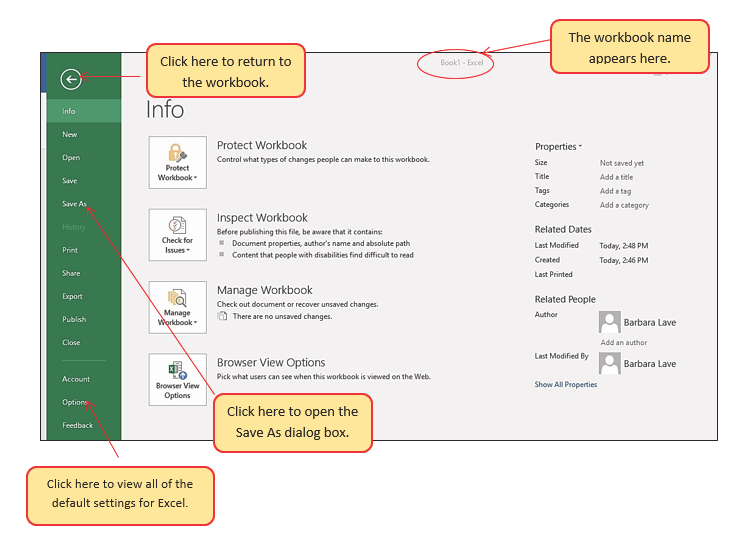
\includegraphics[width=\maxwidth{.95\linewidth}]{gfx/ch01_fig09}
	\caption{File Tab or Backstage View of a Workbook}
	\label{01:fig09}
\end{figure}

The \textit{File} tab includes numerous Excel settings that can be accessed and modified by clicking the \textit{Options} button. Figure \ref{01:fig10} shows the Excel \textit{Options} window, which opens access to settings such as the default font style, font size, and the number of worksheets in new workbooks\footnote{Chapter \ref{ch09:topics}, \nameref{ch09:topics}, page \pageref{ch09:topics}, has more information about setting options.}.

\begin{figure}[H]
	\centering
	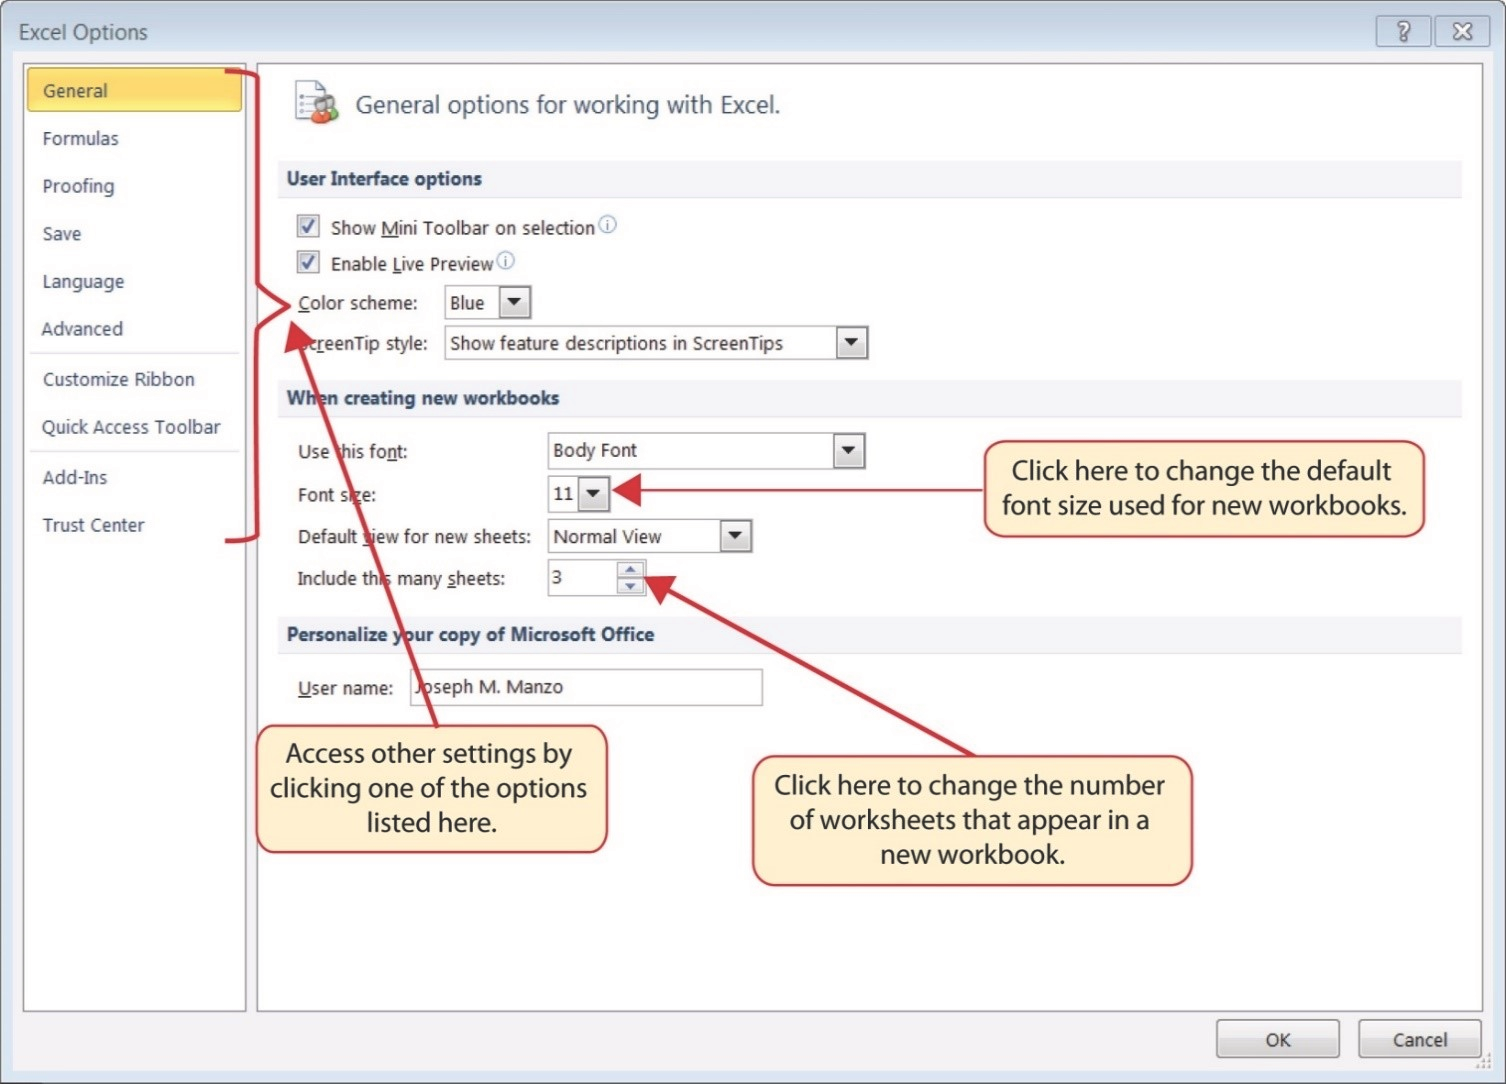
\includegraphics[width=\maxwidth{.95\linewidth}]{gfx/ch01_fig10}
	\caption{Excel Options Window}
	\label{01:fig10}
\end{figure}

\subsection{Saving Workbooks (Save As)}

Once a new workbook is created, the file name and location must be specified on the computer or network. A blank workbook was opened earlier in this lesson and should now be saved. It is important to remember where the workbook is saved since it will be used later in this chapter to construct the workbook shown in Figure \ref{01:fig01}. As a tip, storing all workbooks used in this course in the same folder is probably the easiest.

\begin{enumbox}
	\begin{enumerate}
		\item Click \fmtButton{File $ \Rightarrow $ Save As} to open the \textit{Save As} dialog.
		\item Determine a location for saving on the computer by clicking \fmtButton{Browse} on the left side to open the \textit{Save As} dialog box, as illustrated in Figure \ref{01:fig12}.
	%filesave CH1-GMW Sales Data
		\item Click in the \textit{File Name} box near the bottom of the \textit{Save As} dialog box. Type the new file name: \fmtTyping{CH1-GMW Sales Data}
		\item Review the settings on the screen and click the \fmtButton{Save} button.
	\end{enumerate}
\end{enumbox}

\begin{figure}[H]
	\centering
	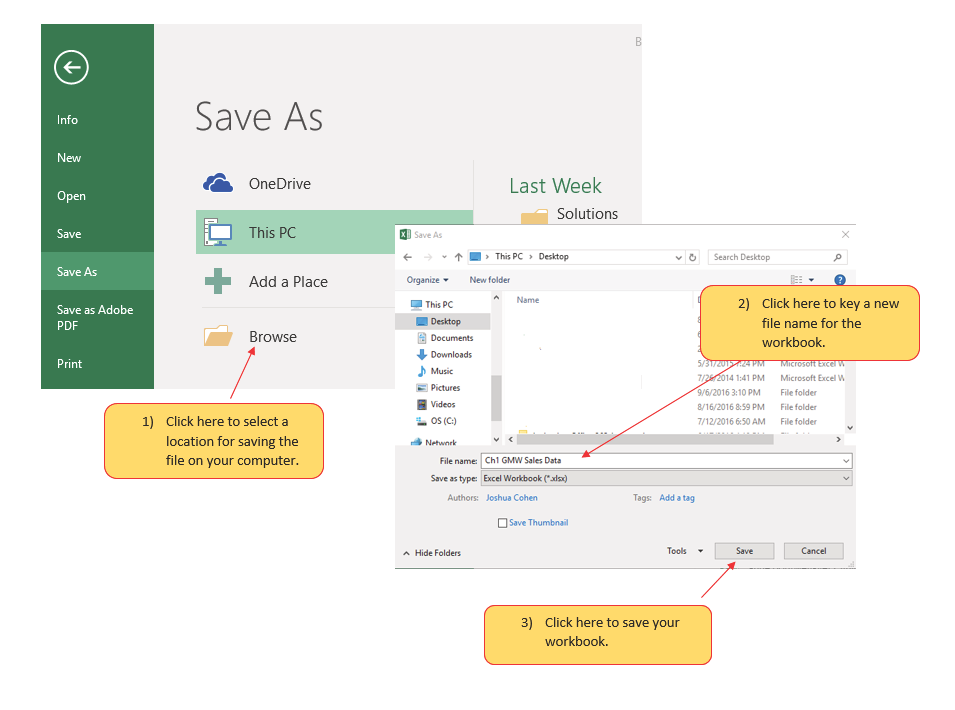
\includegraphics[width=\maxwidth{.95\linewidth}]{gfx/ch01_fig12}
	\caption{Save As Dialog in Excel}
	\label{01:fig12}
\end{figure}

\begin{center}
	\begin{shtcutbox}{Keyboard Shortcuts}
		\textbf{Save As}
		\\
		\begin{itemize}
			\setlength{\itemsep}{0pt}
			\setlength{\parskip}{0pt}
			\setlength{\parsep}{0pt}
			
			\item Tap \fmtKeystroke{F12} and use the tab and arrow keys to navigate around the \textit{Save As} dialog box. Use \fmtKeystroke{Enter} to make a selection.
			\item Or tap \fmtKeystroke{Alt} then \fmtKeystroke{F} and \fmtKeystroke{A} one at a time.
			
		\end{itemize}
	\end{shtcutbox}
\end{center}

\begin{center}
	\begin{sklbox}{Skill Refresher}
		\textbf{Saving Workbooks (Save As)}
		\\
		\begin{itemize}
			\setlength{\itemsep}{0pt}
			\setlength{\parskip}{0pt}
			\setlength{\parsep}{0pt}
			
			\item Click the \textit{File} tab on the Ribbon.
			\item Click the \textit{Save As} option.
			\item Select a location on the computer.
			\item Click in the \textit{File} name box and type a new file name if needed.
			\item Click \textit{Save as type $ \Rightarrow $ Down Arrow} and select the appropriate file type if needed.
			\item Click the \textit{Save} button.
		
		\end{itemize}
	\end{sklbox}
\end{center}

\subsection{The Status Bar}

The Status Bar is located below the worksheet tabs on the Excel screen (see Figure \ref{01:fig13}). It displays various items, such as the status of specific keys on the keyboard (\eg, CAPS LOCK), the available views for a workbook, the magnification of the screen, and mathematical functions that can be performed when data are selected on a worksheet. The Status Bar can be customized as follows.

\begin{enumbox}
	\begin{enumerate}
		\item Place the mouse pointer over any area of the Status Bar and right-click to display the \textit{Customize Status Bar} list of options (see Figure \ref{01:fig13}).
		\item Select the \fmtButton{Caps Lock} option from the menu (see Figure \ref{01:fig13}).
		\item Tap \fmtKeystroke{Caps Lock} and notice the Caps Lock indicator on the lower left side of the Status Bar.
		\item Tap \fmtKeystroke{Caps Lock} a second time and the Status Bar indicator goes away.
	\end{enumerate}
\end{enumbox}

\begin{figure}[H]
	\centering
	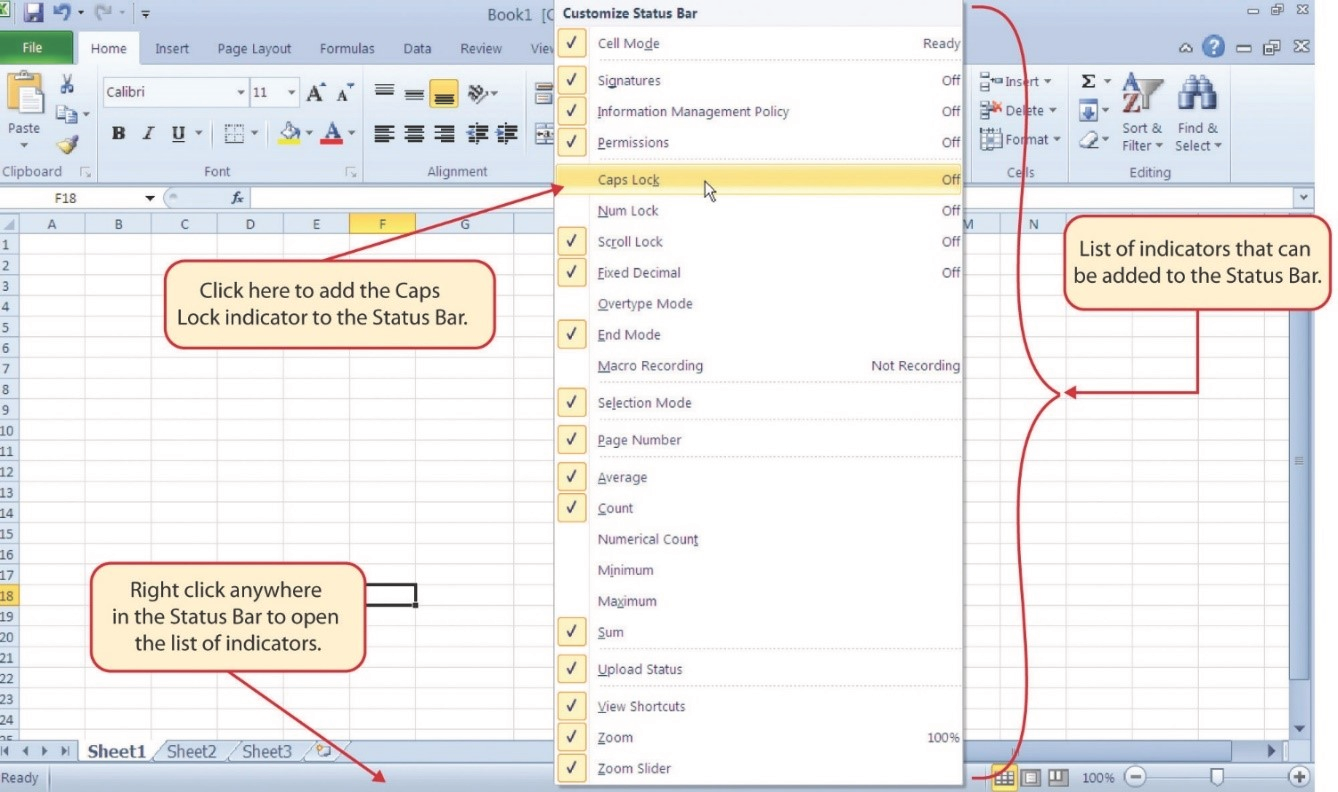
\includegraphics[width=\maxwidth{.95\linewidth}]{gfx/ch01_fig13}
	\caption{Customizing the Status Bar}
	\label{01:fig13}
\end{figure}

\subsection{Excel Help}

The Help feature provides extensive information about the Excel application. Although some of this information may be stored on the local computer, the Help window will automatically connect to the Internet if there is a live connection to provide resources that can answer most questions. 

\fmtOldExcel{Excel 2016} To access help, enter a question in the \textit{Tell me what you want to do} text box above the ribbon. A drop-down list with links to several potential answers will appear. Select from the links or click the question mark to launch the Excel Help window.

\fmtNewExcel{Excel 365} The Excel Help window can be opened by clicking the \fmtButton{Help} tab. Alternatively, enter a question in the \textit{Search} text box above the ribbon. A drop-down list with links to several potential answers will appear. Select from the links or click the question mark to launch the Excel Help window.

\begin{figure}[H]
	\centering
	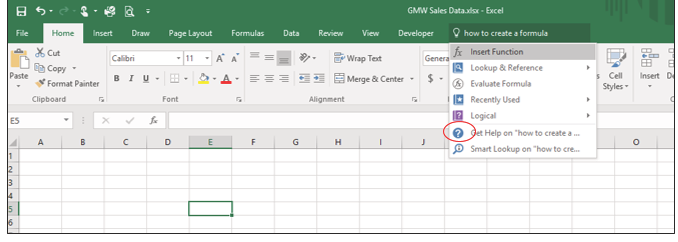
\includegraphics[width=\maxwidth{.95\linewidth}]{gfx/ch01_fig14}
	\caption{Excel Help Window}
	\label{01:fig14}
\end{figure}

\begin{center}
	\begin{shtcutbox}{Keyboard Shortcuts}
		\textbf{Excel Help}
		\\
		\begin{itemize}
			\setlength{\itemsep}{0pt}
			\setlength{\parskip}{0pt}
			\setlength{\parsep}{0pt}
			
			\item Tap \fmtKeystroke{F1}.
			
		\end{itemize}
	\end{shtcutbox}
\end{center}


\begin{center}
	\begin{tkwbox}{Key Take-Aways}
		\textbf{Overview}
		\\
		\begin{itemize}
			\setlength{\itemsep}{0pt}
			\setlength{\parskip}{0pt}
			\setlength{\parsep}{0pt}
			
			\item Excel is a powerful tool for processing data to make decisions.
			\item Excel commands are found throughout the tabs in the Ribbon.
			\item The \textit{Quick Access Toolbar} can be customized by adding frequently-used commands.
			\item The information displayed on the Status Bar can be customized.
			\item The Help window provides extensive information about Excel.
			
		\end{itemize}
	\end{tkwbox}
\end{center}

\section{Entering, Editing, and Managing Data}

\begin{center}
	\begin{objbox}{Learning Objectives}
		\begin{itemize}
			\setlength{\itemsep}{0pt}
			\setlength{\parskip}{0pt}
			\setlength{\parsep}{0pt}
			
			\item Understand how to enter data into a worksheet.
			\item Examine how to edit data in a worksheet.
			\item Examine how \textit{AutoFill} is used when entering data.
			\item Understand how to delete data from a worksheet and use the Undo command.
			\item Examine how to adjust column widths and row heights in a worksheet.
			\item Understand how to hide columns and rows in a worksheet.
			\item Examine how to insert columns and rows into a worksheet.
			\item Understand how to delete columns and rows from a worksheet.
			\item Learn how to move data to different locations in a worksheet.

		\end{itemize}
	\end{objbox}
\end{center}

This section begins the development of the workbook shown in Figure \ref{01:fig01}. The skills covered in this section are typically used in the early stages of developing one or more worksheets in a workbook.

\subsection{Entering Data}

Begin building the workbook shown in Figure \ref{01:fig01} by manually entering data into the worksheet. Begin by entering the column headings in \textit{Row 2}.

\begin{enumbox}
	\begin{enumerate}
		\item Click cell location \fmtLoc{A2} on the worksheet.
		\item Type the word \fmtTyping{Month}.
		\item Tap \fmtKeystroke{Tab} to enter the word into cell \fmtLoc{A2} and activate the next cell to the right.
		\item Type \fmtTyping{Unit Sales}, then tap \fmtKeystroke{Tab}.
		\item Repeat the above step for the words \fmtTyping{Average Price} and then again for \fmtTyping{Sales Dollars}.
	\end{enumerate}
\end{enumbox}
	
Figure \ref{01:fig15} shows how the worksheet should appear after entering the column headings into \textit{Row 2}. Notice that the word \textit{Price} in cell location $ C2 $ is not visible because the column is too narrow to fit the entry. This formatting will be corrected in the next section.

\begin{figure}[H]
	\centering
	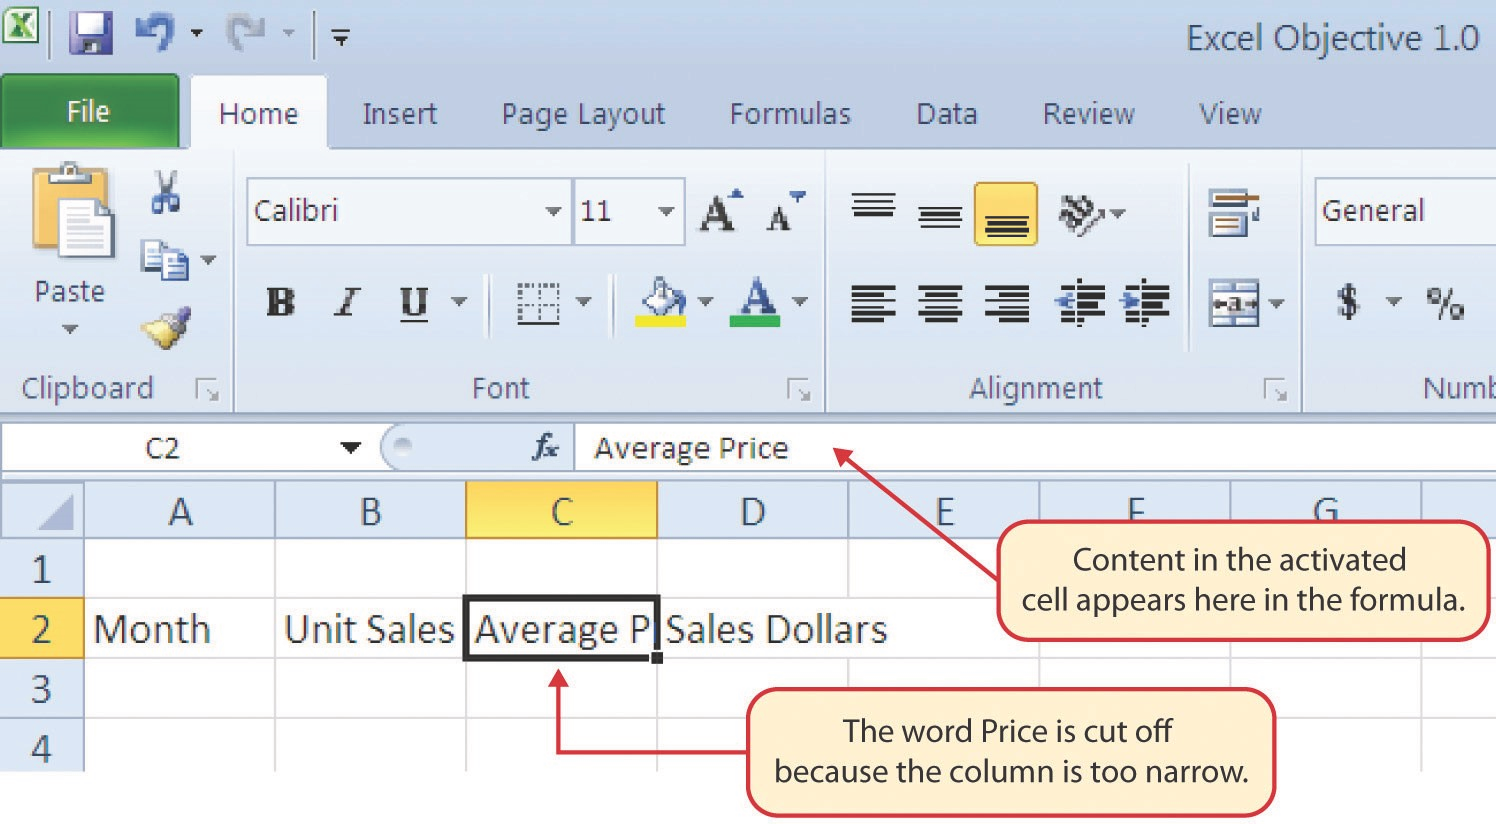
\includegraphics[width=\maxwidth{.95\linewidth}]{gfx/ch01_fig15}
	\caption{Entering Column Headings into a Worksheet}
	\label{01:fig15}
\end{figure}

\begin{center}
	\begin{infobox}{Integrity Check}
		\textbf{Column Headings}
		\\
		\\
		It is critical to include column headings that accurately describe the data in each worksheet column. In professional environments, Excel workbooks are commonly shared among coworkers. Good column headings reduce the chance of someone misinterpreting the data contained in a worksheet, leading to costly errors.
	\end{infobox}
\end{center}

\begin{enumbox}
	\begin{enumerate}
		\item Click cell location \fmtLoc{B3}.
		\item Type the number \fmtTyping{$ 2670 $}, then tap \fmtKeystroke{Enter}. After tapping \fmtKeystroke{Enter}, cell \fmtLoc{B4} will be activated. Using \fmtKeystroke{Enter} is an efficient way to enter data vertically down a column.
		\item Enter the following numbers in cells \fmtLoc{B4} through \fmtLoc{B14}: \fmtTyping{$ 2160 $}, \fmtTyping{$ 515 $}, \fmtTyping{$ 590 $}, \fmtTyping{$ 1030 $}, \fmtTyping{$ $ 2875 $ $}, \fmtTyping{$ 2700 $}, \fmtTyping{$ 900 $}, \fmtTyping{$ 775 $}, \fmtTyping{$ 1180 $}, \fmtTyping{$ 1800 $}, and \fmtTyping{$ 3560 $}.
		\item Click cell location \fmtLoc{C3}.
		\item Type the number \fmtTyping{$ 9.99 $}, then tap \fmtKeystroke{Enter}.
		\item Enter the following numbers in cells \fmtLoc{C4} through \fmtLoc{C14}: \fmtTyping{$ 12.49 $}, \fmtTyping{$ 14.99 $}, \fmtTyping{$ 17.49 $}, \fmtTyping{$ 14.99 $}, \fmtTyping{$ 12.49 $}, \fmtTyping{$ 9.99 $}, \fmtTyping{$ 19.99 $}, \fmtTyping{$ 19.99 $}, \fmtTyping{$ 19.99 $}, \fmtTyping{$ 17.49 $}, and \fmtTyping{$ 14.99 $}.
		\item Click in cell \fmtLoc{D3}.
		\item Type the number \fmtTyping{$ 26685 $}, then tap \fmtKeystroke{Enter}.
		\item Enter the following numbers in cells \fmtLoc{D4} through \fmtLoc{D14}: \fmtTyping{$ 26937 $}, \fmtTyping{$ 7701 $}, \fmtTyping{$ 10269 $}, \fmtTyping{$ 15405 $}, \fmtTyping{$ 35916 $}, \fmtTyping{$ 26937 $}, \fmtTyping{$ 17958 $}, \fmtTyping{$ 15708 $}, \fmtTyping{$ 23562 $}, \fmtTyping{$ 31416 $}, and \fmtTyping{$ 53370 $}.
		\item When finished, check that the data entered matches Figure \ref{01:fig16}.
	\end{enumerate}
\end{enumbox}
	
\begin{figure}[H]
	\centering
	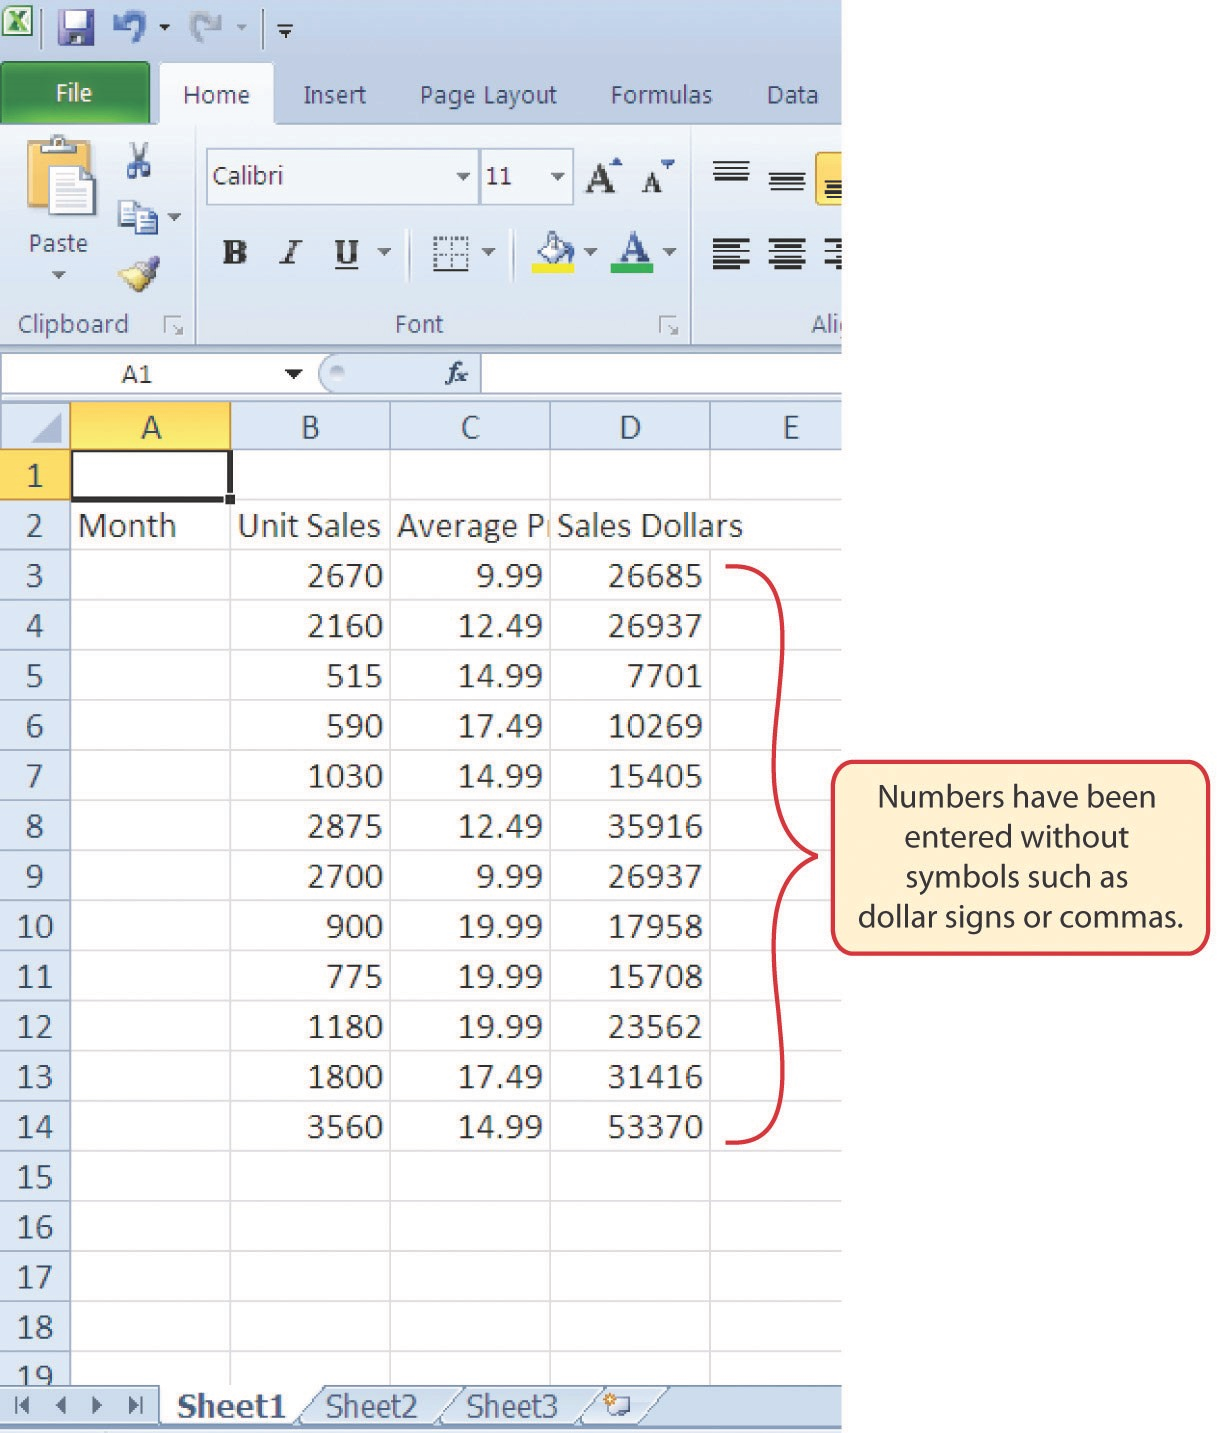
\includegraphics[width=\maxwidth{.95\linewidth}]{gfx/ch01_fig16}
	\caption{Completed Data Entry for Columns B, C, and D}
	\label{01:fig16}
\end{figure}

\begin{center}
	\begin{infobox}{Integrity Check}
		\textbf{Data Entry}
		\\
		\\
		One of the most likely points of error in any spreadsheet project is inaccurate data entry. It is easy to transpose or skip digits when entering a row of numbers. Carefully checking data entry will reduce confusing results during the analysis phase of the project.
	\end{infobox}
\end{center}

\begin{center}
	\begin{infobox}{Why?}
		\textbf{Avoid Formatting Symbols When Entering Numbers}
		\\
		\\
		When typing numbers into an Excel worksheet, it is best to avoid adding formatting symbols such as dollar signs and commas. Although Excel allows these symbols to be included while typing numbers, it slows down the process of entering data. It is more efficient to use Excel's formatting features to add these symbols to numbers after they are typed into a worksheet.
	\end{infobox}
\end{center}

\subsection{Editing Data}

Data entered in a cell can be changed by double-clicking the cell location or using the Formula Bar. The Formula Bar can be used for the initial entry of data into cells and for editing data that already exists in a cell. The following steps provide an example of entering and editing data entered into a cell location.

\begin{enumbox}
	\begin{enumerate}
		\item Click cell \fmtLoc{A15} in the \fmtWorksheet{Sheet1} worksheet.
		\item Type the abbreviation \fmtTyping{Tot}, then tap \fmtKeystroke{Enter}.
		\item Click cell \fmtLoc{A15}.
		\item Move the mouse pointer up to the Formula Bar. Notice that the pointer turns into a cursor. Move the cursor to the end of the abbreviation \textit{Tot} and left-click.
		\item Type the letters \fmtTyping{al} to complete the word \textit{Total}.
		\item Click the checkmark to the left of the Formula Bar (see Figure \ref{01:fig17}) or tap \fmtKeystroke{Enter} to enter the change into the cell.
	
		\begin{figure}[H]
			\centering
			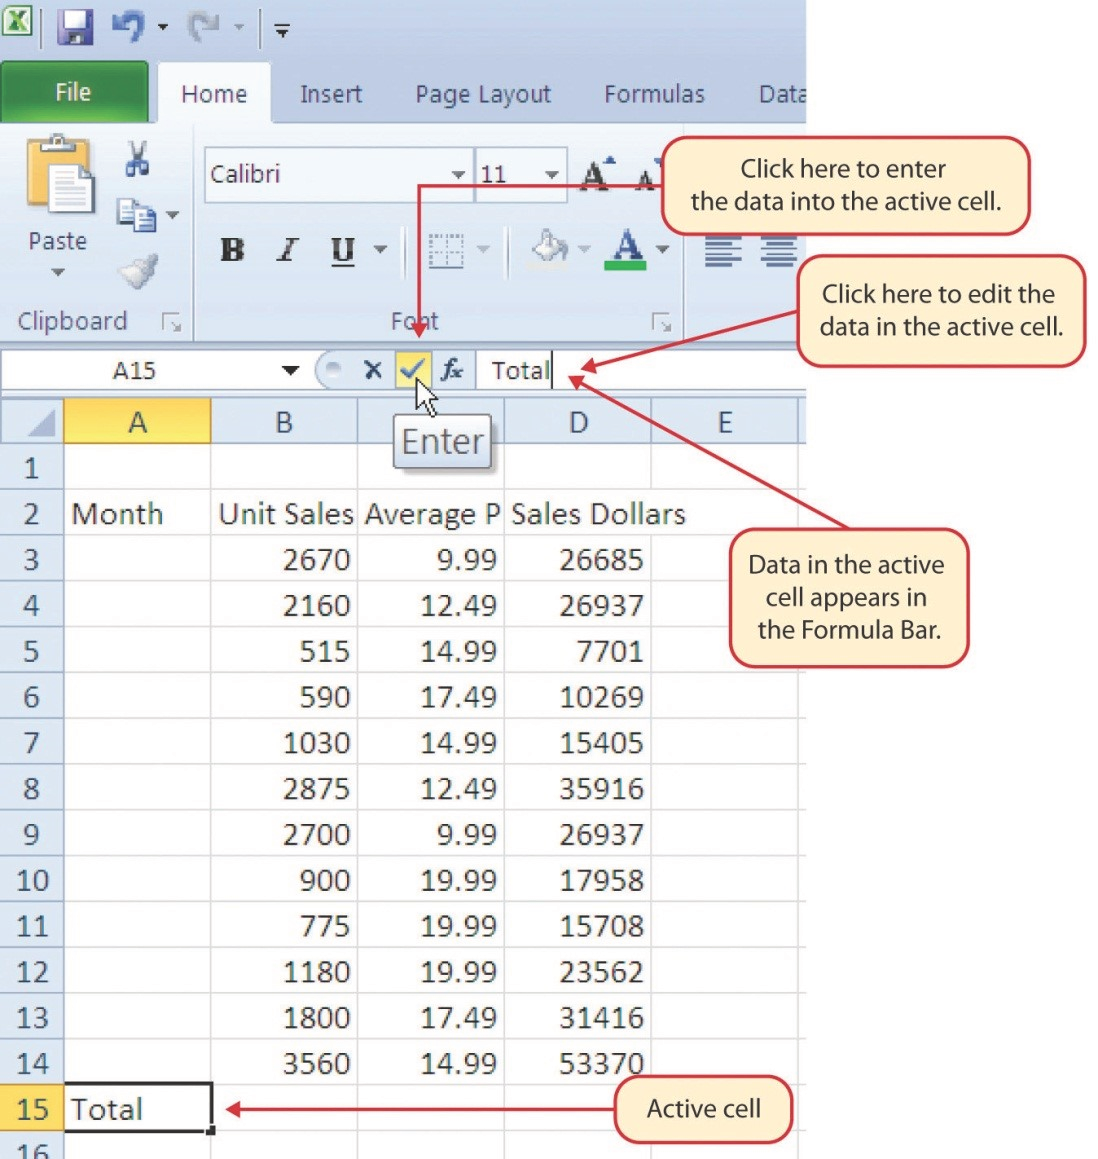
\includegraphics[width=\maxwidth{.95\linewidth}]{gfx/ch01_fig17}
			\caption{Using the Formula Bar to Edit and Enter Data}
			\label{01:fig17}
		\end{figure}

		\item Double click cell \fmtLoc{A15}.
		\item Add a space after the word \textit{Total} and type the word \fmtTyping{Sales}.
		\item Tap \fmtKeystroke{Enter}.
	\end{enumerate}
\end{enumbox}
	
\begin{center}
	\begin{shtcutbox}{Keyboard Shortcuts}
		\textbf{Editing Data in a Cell}
		\\
		\begin{itemize}
			\setlength{\itemsep}{0pt}
			\setlength{\parskip}{0pt}
			\setlength{\parsep}{0pt}
			
			\item Click in the cell that is to be edited, then tap \fmtKeystroke{F2}. Alternatively, double-click the cell to be edited.
			
		\end{itemize}
	\end{shtcutbox}
\end{center}

\subsection{AutoFill}

\textit{AutoFill} is a valuable feature when manually entering data into a worksheet. \textit{AutoFill} is most beneficial when entering data with a defined sequence, such as the numbers $ 2 $, $ 4 $, $ 6 $, $ 8 $, or the months of the year. The following steps demonstrate how \textit{AutoFill} can be used to enter the months of the year in \textit{Column A}.

\begin{enumbox}
	\begin{enumerate}
		\item Click cell \fmtLoc{A3} in the \fmtWorksheet{Sheet1} worksheet.
		\item Type the word \fmtTyping{January}, then tap \fmtKeystroke{Enter}.
		\item Click in cell \fmtLoc{A3} again.
		\item Move the mouse pointer to the lower right corner of cell \fmtLoc{A3}. Notice a small square called the \textit{AutoFill Handle} (See Figure \ref{01:fig18}). When the mouse pointer gets close to the \textit{AutoFill Handle}, the pointer's white block plus sign will turn into a black plus sign.

		\begin{figure}[H]
			\centering
			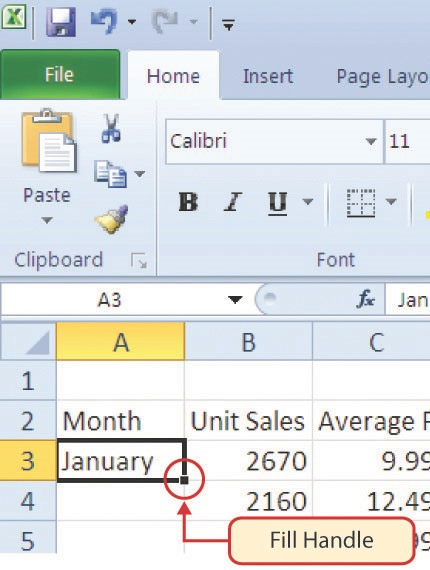
\includegraphics[width=\maxwidth{.75\linewidth}]{gfx/ch01_fig18}
			\caption{AutoFill Handle}
			\label{01:fig18}
		\end{figure}

		\item Left-click and drag the \textit{AutoFill Handle} to cell \fmtLoc{A14}. Notice that the \textit{AutoFill Handle} tip box indicates what month will be placed into each cell (see Figure \ref{01:fig19}). Release the left mouse button when the tip box reads \textit{December}.
	\end{enumerate}
\end{enumbox}
	
\begin{figure}[H]
	\centering
	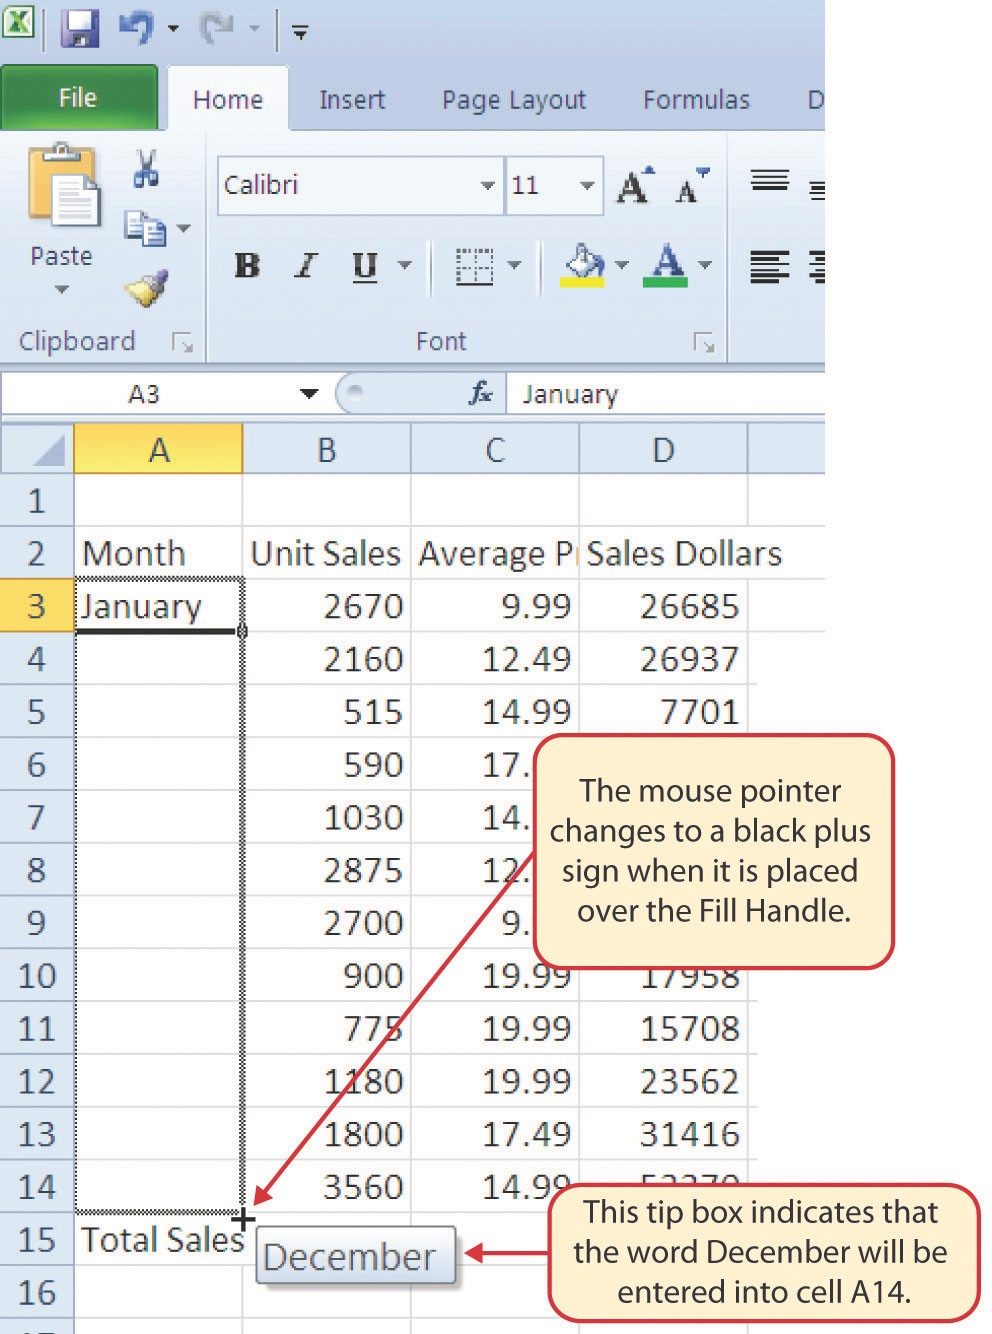
\includegraphics[width=\maxwidth{.95\linewidth}]{gfx/ch01_fig19}
	\caption{Using AutoFill Handle to Enter the Months of the Year}
	\label{01:fig19}
\end{figure}

Once the left mouse button is released, all twelve months of the year should appear in the cell range $ A3 $:$ A14 $, as shown in Figure \ref{01:fig20}. After auto-filling a range, an \textit{Auto Fill Options} button pops up at the lower right corner of the filled range, as shown in Figure \ref{01:fig20}. 

\fmtOldExcel{Excel 2016} The \textit{AutoFill Options} button presents several options for changing how the range is filled.

\begin{figure}[H]
	\centering
	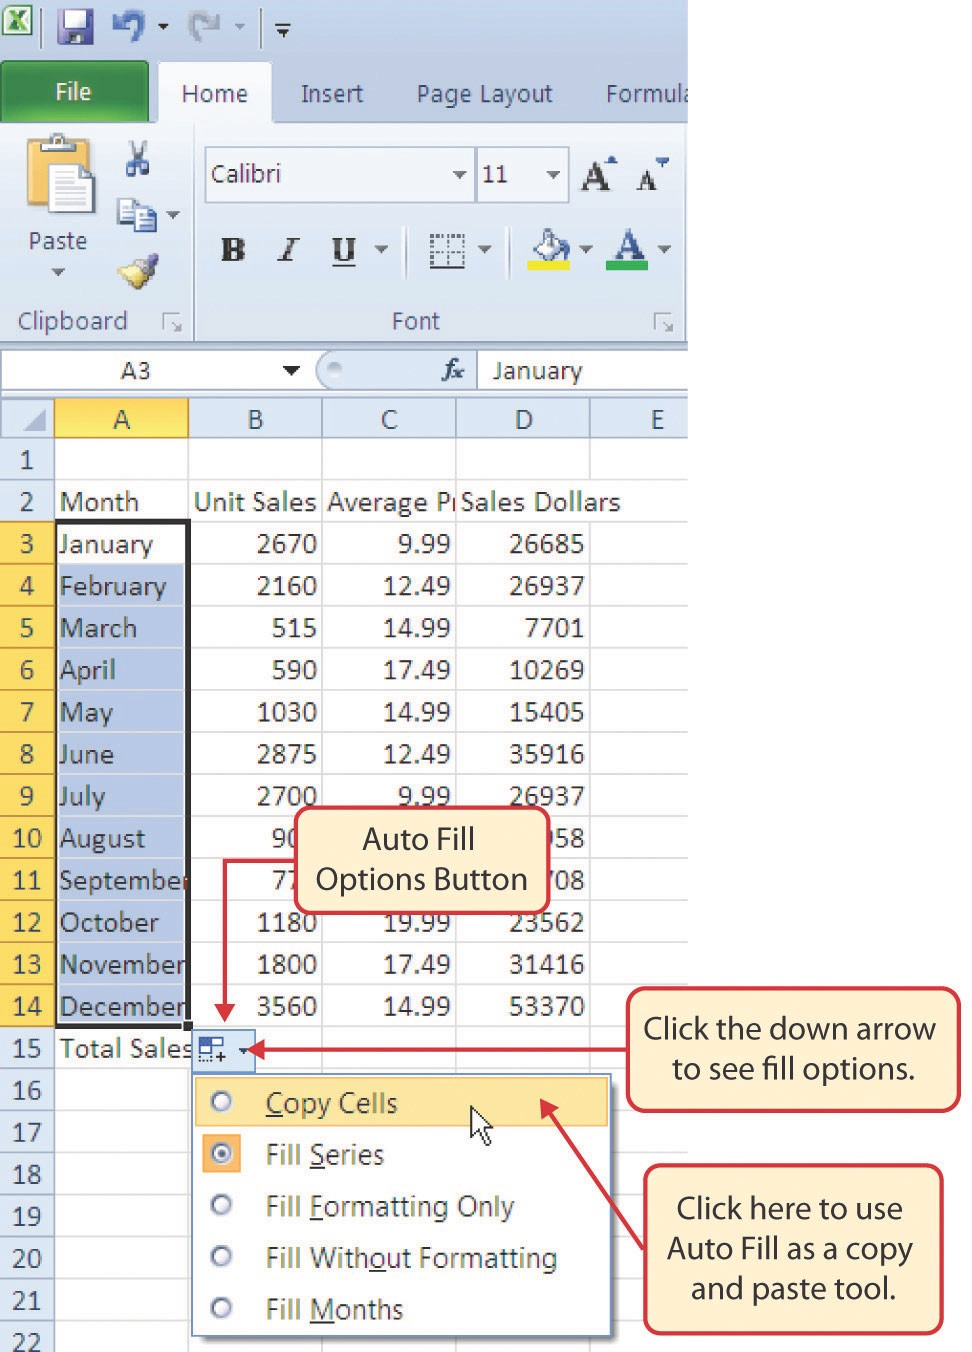
\includegraphics[width=\maxwidth{.95\linewidth}]{gfx/ch01_fig20}
	\caption{AutoFill Options Button}
	\label{01:fig20}
\end{figure}

\begin{enumbox}
	\begin{enumerate}
		\item Click the \textit{AutoFill Options} button.
		\item Click the \fmtButton{Copy Cells} option to change the months in  \fmtLoc{A4:A14} to January.
		\item Click the \textit{AutoFill Options} button again.
		\item Click the \fmtButton{Fill Months} option to return the months of the year to the cell range \fmtLoc{A4:A14}. The \fmtButton{Fill Series} option will provide the same result.
	\end{enumerate}
\end{enumbox}

\fmtNewExcel{Excel 365} The \textit{AutoFill Options} button was replaced with the \textit{Quick Analysis} button. That button will apply several possible analysis features to the filled range, like highlighting duplicated entries.

\begin{figure}[H]
	\centering
	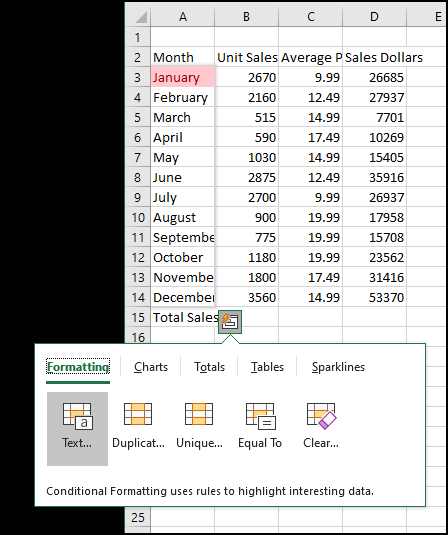
\includegraphics[width=\maxwidth{.95\linewidth}]{gfx/ch01_fig20a}
	\caption{Quick Analysis Button}
	\label{01:fig20a}
\end{figure}

\begin{enumbox}
	\begin{enumerate}
		\item Click the \fmtButton{Quick Analysis} button.
		\item Hover the mouse over each Format tab option and notice how the text in the cells is selected.
		\item Click anywhere in the worksheet to finish the \textit{AutoFill} process.
	\end{enumerate}
\end{enumbox}

\subsection{Deleting Data and the Undo Command}

There are several methods for removing data from a worksheet, a few of which are demonstrated here. With each method, use the \textit{Undo} command to return the deleted data. Undo is available on the Quick Access Toolbar or the keyboard shortcut: press and hold \fmtKeystroke{Ctrl}, then tap \fmtKeystroke{Z}. Undo is a helpful command if data is mistakenly deleted from the worksheet. The following steps demonstrate how to delete data from a cell or range of cells.

\begin{enumbox}
	\begin{enumerate}
		\item Click cell \fmtLoc{C2} by placing the mouse pointer over the cell and clicking the left mouse button.
		\item Tap \fmtKeystroke{Delete} to remove the contents of the cell.
		\item Select \fmtLoc{C3:C14} by placing the mouse pointer over cell \fmtLoc{C3}, then left-click and drag the mouse pointer down to cell \fmtLoc{C14}.
		\item Place the mouse pointer over the \textit{AutoFill Handle}. Notice that the white block plus sign changed to a black plus sign.
		\item Click and drag the mouse pointer up to cell \fmtLoc{C3}, as in Figure \ref{01:fig21}. Release the mouse button. The contents in \fmtLoc{C3:C14} will be removed.
	\end{enumerate}
\end{enumbox}

\begin{figure}[H]
	\centering
	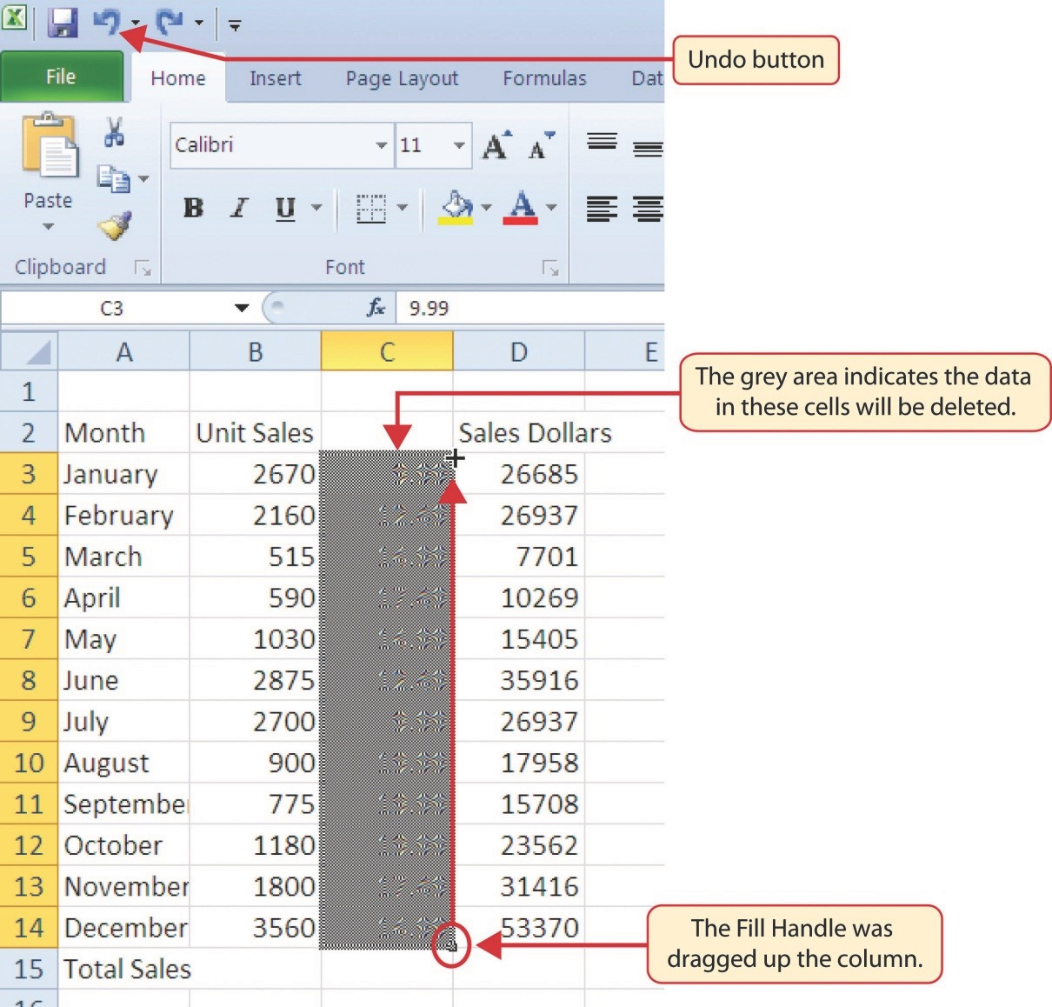
\includegraphics[width=\maxwidth{.95\linewidth}]{gfx/ch01_fig21}
	\caption{Using AutoFill to Delete Contents of Cell}
	\label{01:fig21}
\end{figure}

\begin{enumbox}
	\begin{enumerate}
		\item Click the \fmtButton{Undo} button in the \fmtButton{Quick Access Toolbar}, as illustrated in Figure \ref{01:fig21}, to replace the data in \fmtLoc{C3:C14}.
		\item Click the \fmtButton{Undo} button again to replace the data in cell \fmtLoc{C2}.
	\end{enumerate}
\end{enumbox}

\begin{center}
	\begin{shtcutbox}{Keyboard Shortcuts}
		\textbf{Undo Command}
		\\
		\begin{itemize}
			\setlength{\itemsep}{0pt}
			\setlength{\parskip}{0pt}
			\setlength{\parsep}{0pt}
			
			\item Press and hold \fmtKeystroke{Ctrl}, then tap \fmtKeystroke{Z}.
			
		\end{itemize}
	\end{shtcutbox}
\end{center}

\begin{enumbox}
	\begin{enumerate}
		\item Select \fmtLoc{C2:C14} by placing the mouse pointer over cell \fmtLoc{C2}. Then left-click and drag the mouse pointer down to cell \fmtLoc{C14}.
		\item Click \fmtButton{Home $ \Rightarrow $ Editing $ \Rightarrow $ Clear} (see Figure \ref{01:fig22}) to open a drop-down menu with several options for removing or clearing data from a cell. Notice that there are also options for clearing just the formats or the hyperlinks in a cell.
		\item Click the \fmtButton{Clear All} to remove the data in the cell range.
		\item Click the \fmtButton{Undo} button to replace the data in \fmtLoc{C2:C14}.
	\end{enumerate}
\end{enumbox}

\begin{figure}[H]
	\centering
	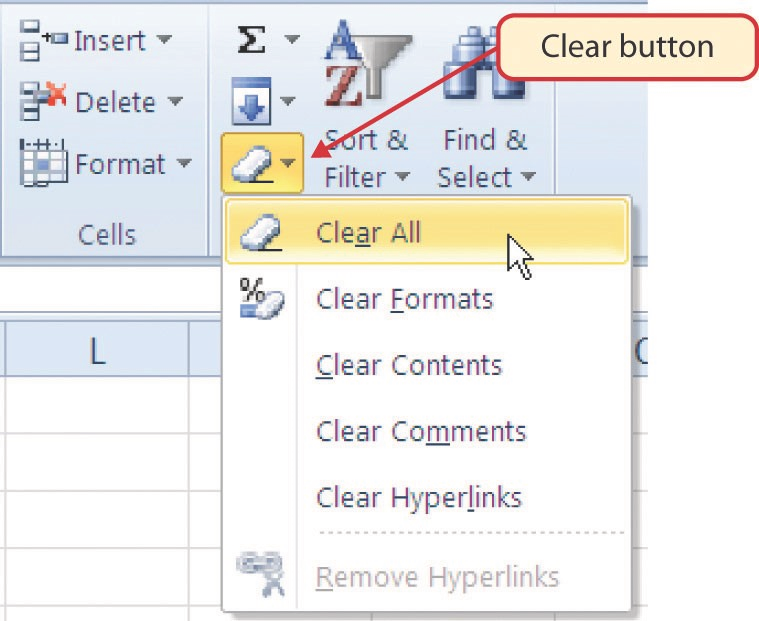
\includegraphics[width=\maxwidth{.95\linewidth}]{gfx/ch01_fig22}
	\caption{Clear Command Drop-Down Menu}
	\label{01:fig22}
\end{figure}

\subsection{Adjusting Columns and Rows}

A few entries in the worksheet appear to be cut off. For example, the last letter of the word \textit{September} cannot be seen in cell $ A11 $ since the column is too narrow for the word. The columns and rows on an Excel worksheet can be adjusted to accommodate the data entered into a cell. The following steps explain adjusting the worksheet's column widths and row heights.

\begin{enumbox}
	\begin{enumerate}
		\item Bring the mouse pointer between \fmtLoc{Column A} and \fmtLoc{Column B} in the \fmtWorksheet{Sheet1} worksheet, as shown in Figure \ref{01:fig23}. Notice that the pointer's white block plus sign turns into double arrows.
		\item Click and drag the column to the right, so the entire word \textit{September} in cell \fmtLoc{A11} can be seen. As the column separator is dragged to the right, the column width pops up in a tip box. This box displays the number of characters that will fit into the column using the Calibri 11-point font, the default setting for font/size.
		\item Release the left mouse button.
	\end{enumerate}
\end{enumbox}
	
\begin{figure}[H]
	\centering
	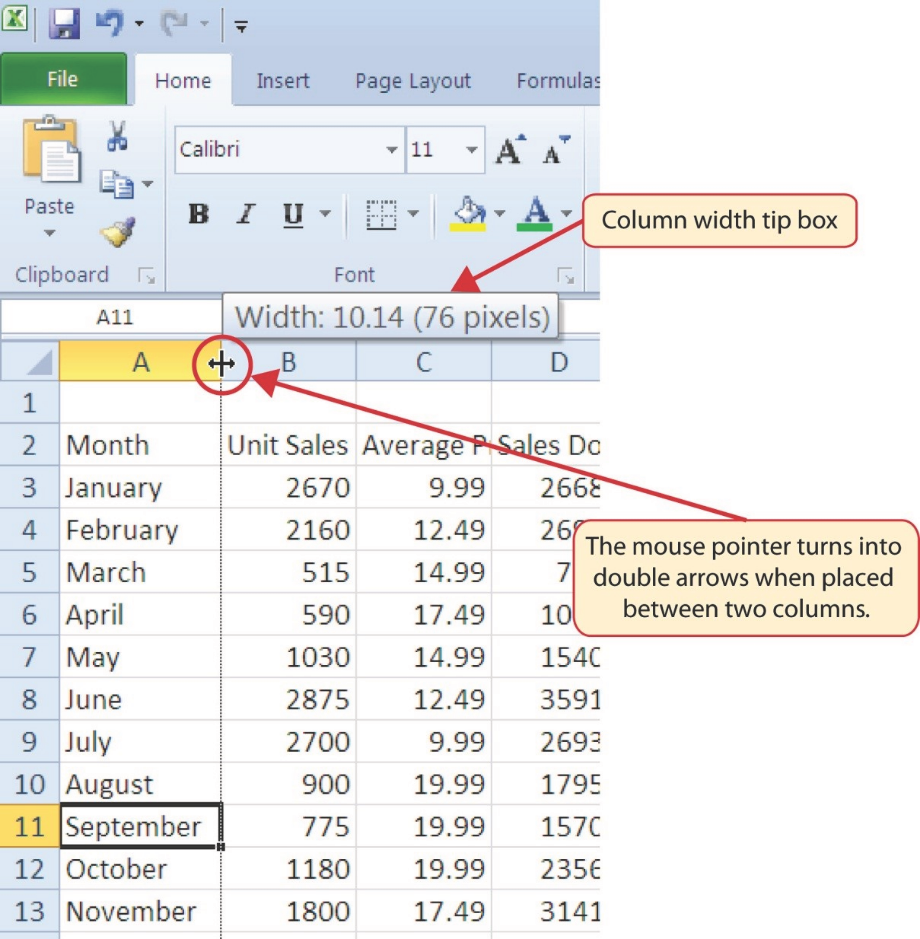
\includegraphics[width=\maxwidth{.95\linewidth}]{gfx/ch01_fig23}
	\caption{Adjusting Column Widths}
	\label{01:fig23}
\end{figure}

The click-and-drag method can be inefficient in setting a specific character width for more than one column. The following steps illustrate a second method for adjusting columns to a specific width.

\begin{enumbox}
	\begin{enumerate}
		\item Click any cell location in \fmtLoc{Column A} by moving the mouse pointer over a cell location and clicking the left mouse button. 
		\item Click \fmtButton{Home $ \Rightarrow $ Cells $ \Rightarrow $ Format $ \Rightarrow $ Column Width} to open the \textit{Column Width} dialog box.
		\item Type the number \fmtTyping{13} and click the \fmtButton{OK} button on the \textit{Column Width} dialog box to set \fmtLoc{Column A} to display $ 13 $ characters based on the default font (see Figure \ref{01:fig24}).
		\item As a third option, bring the mouse pointer between \fmtLoc{Column A} and \fmtLoc{Column B} so that the double arrow pointer displays and then double-click. This process activates \fmtButton{AutoFit} to adjust the column width based on the most extended entry in the column.
		\item Use the \textit{Column Width} dialog box to set the width to \fmtTyping{13}.
	\end{enumerate}
\end{enumbox}
	
\begin{figure}[H]
	\centering
	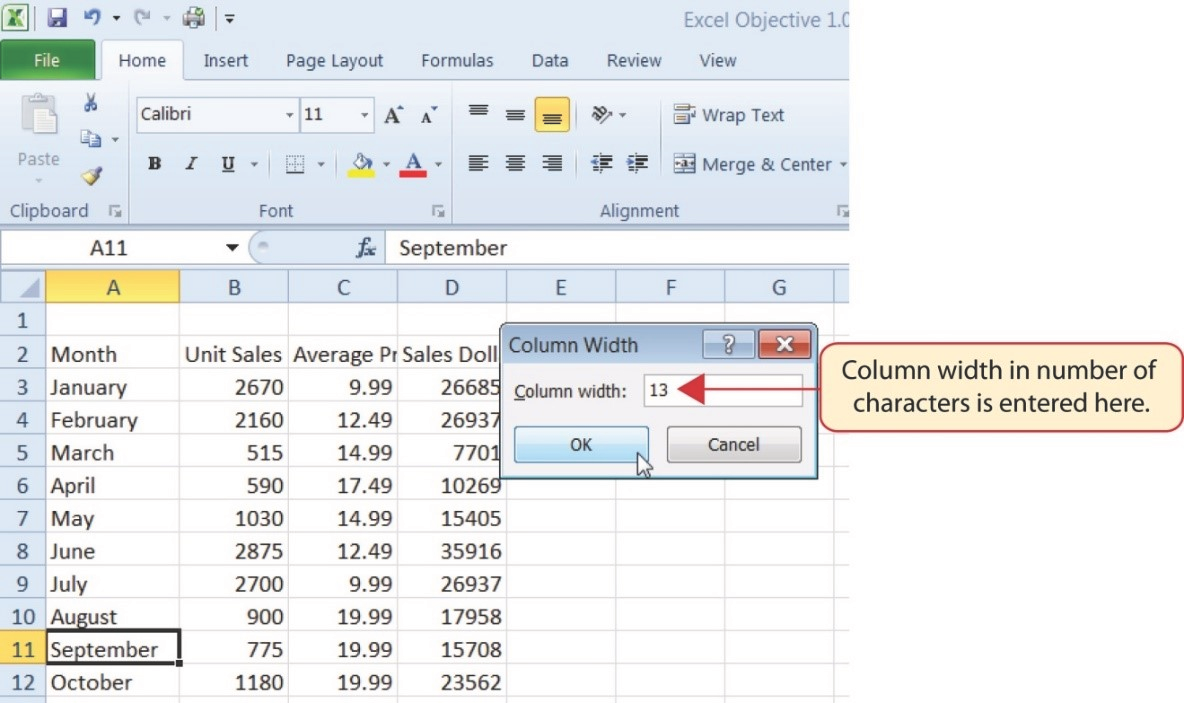
\includegraphics[width=\maxwidth{.95\linewidth}]{gfx/ch01_fig24}
	\caption{Column Width Dialog Box}
	\label{01:fig24}
\end{figure}

\begin{center}
	\begin{shtcutbox}{Keyboard Shortcuts}
		\textbf{Column Width}
		\\
		\begin{itemize}
			\setlength{\itemsep}{0pt}
			\setlength{\parskip}{0pt}
			\setlength{\parsep}{0pt}
			
			\item Tap \fmtKeystroke{Alt} and then tap the letters \fmtKeystroke{H}, \fmtKeystroke{O}, and \fmtKeystroke{W} one at a time.
			
		\end{itemize}
	\end{shtcutbox}
\end{center}

The following steps demonstrate how to adjust row height.

\begin{enumbox}
	\begin{enumerate}
		\item Click cell \fmtLoc{A15}.
		\item Click \fmtButton{Home $ \Rightarrow $ Cells $ \Rightarrow $ Format $ \Rightarrow $ Row Height} to open the \textit{Row Height} dialog box.
		\item Type the number \fmtTyping{24} and click the \fmtButton{OK} button on the \textit{Row Height} dialog box to set \fmtLoc{Row 15} to a height of $ 24 $ points. A point is equivalent to approximately $ 1/72 $ of an inch. This adjustment was made to create space between the worksheet totals and the other data.
		\item Row height can also be adjusted by dragging the border between \fmtLoc{Row 15} and \fmtLoc{Row 16} or by double-clicking the border between \fmtLoc{Row 15} and \fmtLoc{Row 16}.
	\end{enumerate}
\end{enumbox}

\begin{center}
	\begin{shtcutbox}{Keyboard Shortcuts}
		\textbf{Column Width}
		\\
		\begin{itemize}
			\setlength{\itemsep}{0pt}
			\setlength{\parskip}{0pt}
			\setlength{\parsep}{0pt}
			
			\item Tap \fmtKeystroke{Alt} then tap the letters \fmtKeystroke{H}, \fmtKeystroke{O}, and \fmtKeystroke{H} one at a time.
			
		\end{itemize}
	\end{shtcutbox}
\end{center}

Figure \ref{01:fig25} shows the appearance of the worksheet after adjusting  \fmtLoc{Column A} and \fmtLoc{Row 15}.

\begin{figure}[H]
	\centering
	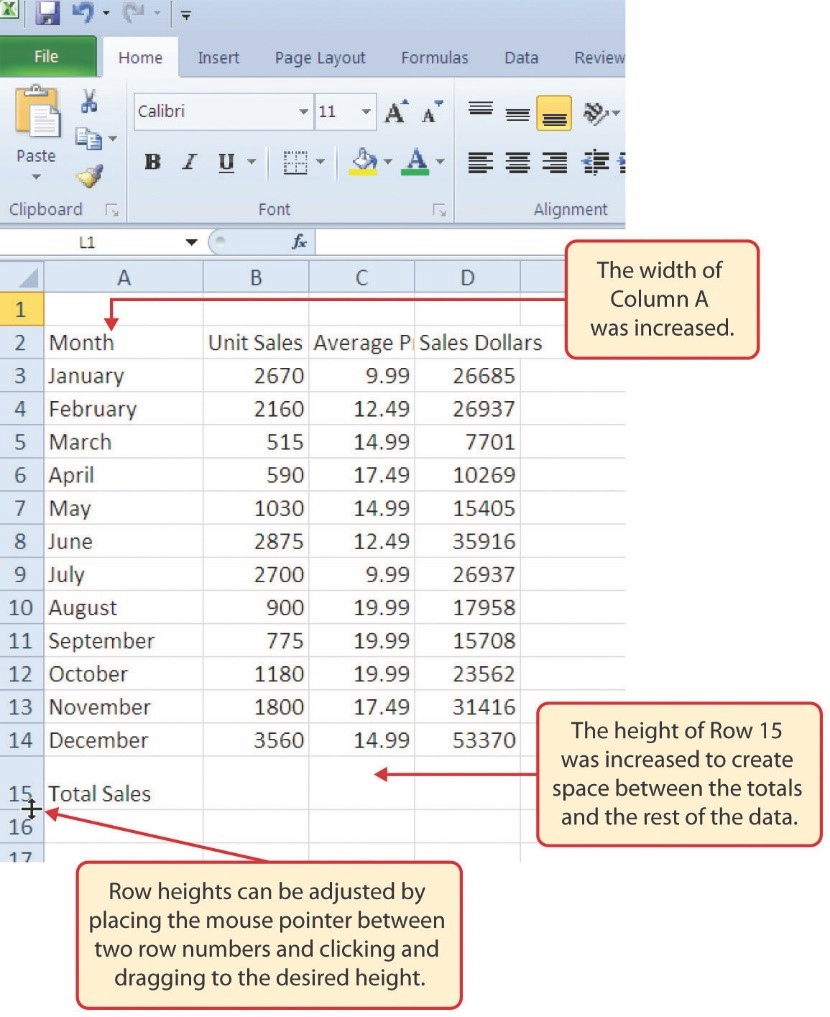
\includegraphics[width=\maxwidth{.95\linewidth}]{gfx/ch01_fig25}
	\caption{CH1-GMW Sales Data with Column A and Row 15 Adjusted}
	\label{01:fig25}
\end{figure}

\begin{center}
	\begin{sklbox}{Skill Refresher}
		\textbf{Adjusting Columns and Rows}
		\\
		\begin{itemize}
			\setlength{\itemsep}{0pt}
			\setlength{\parskip}{0pt}
			\setlength{\parsep}{0pt}
			
			\item Activate at least one cell in the row or column being adjusted.
			\item Click \textit{Home $ \Rightarrow $ Cells $ \Rightarrow $ Format}
			\item Click either \textit{Row Height} or \textit{Column Width} from the drop-down menu.
			\item Enter the Row Height in points or Column Width in characters in the dialog box.
			\item Click the \textit{OK} button.
			
		\end{itemize}
	\end{sklbox}
\end{center}

\subsection{Hiding Columns and Rows}

In addition to adjusting the columns and rows on a worksheet, they can also be hidden. Hiding columns is a valuable technique for enhancing the visual appearance when it includes data that is not necessary to display. Later in the course, these features will be demonstrated using the \textit{CH1-GMW Sales Data} workbook; however, this worksheet does not need to have hidden columns or rows. The use of these skills will be presented here for demonstration purposes only.

\begin{enumbox}
	\begin{enumerate}
		\item Click cell \fmtLoc{C1} in the \fmtWorksheet{Sheet1} worksheet.
		\item Click \fmtButton{Home $ \Rightarrow $ Cells $ \Rightarrow $ Format $ \Rightarrow $ Hide \& Unhide} to open a submenu of options.
		\item Click the \fmtButton{Hide Columns} option in the submenu of options (see Figure \ref{01:fig26}) to hide \fmtLoc{Column C}.
	\end{enumerate}
\end{enumbox}

\begin{figure}[H]
	\centering
	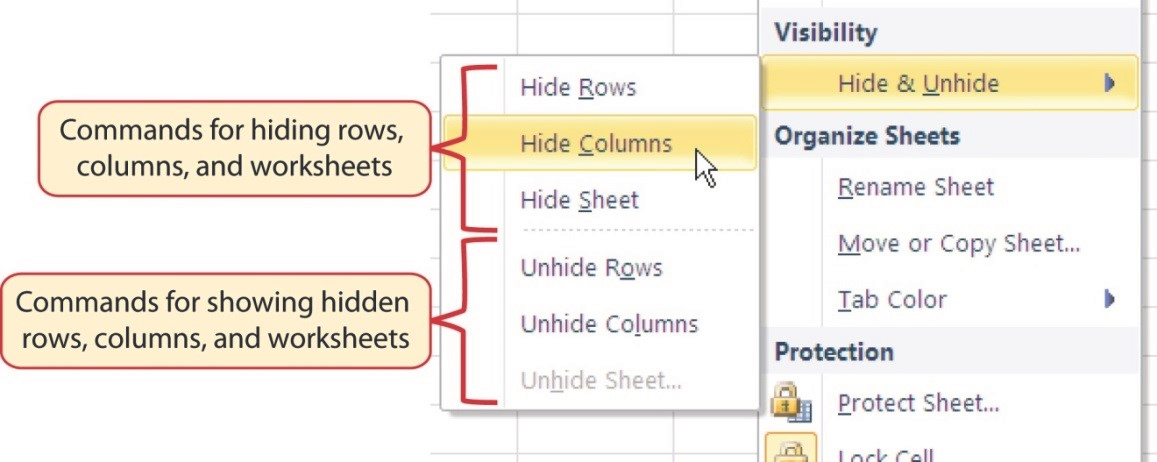
\includegraphics[width=\maxwidth{.95\linewidth}]{gfx/ch01_fig26}
	\caption{Hide \& Unhide Submenu}
	\label{01:fig26}
\end{figure}

\begin{center}
	\begin{shtcutbox}{Keyboard Shortcuts}
		\textbf{Hiding Columns}
		\\
		\begin{itemize}
			\setlength{\itemsep}{0pt}
			\setlength{\parskip}{0pt}
			\setlength{\parsep}{0pt}
			
			\item Press and hold \fmtKeystroke{Ctrl}, then tap \fmtKeystroke{0}. (Note, this is the number zero, not the letter O.)
			
		\end{itemize}
	\end{shtcutbox}
\end{center}

Figure \ref{01:fig27} shows the workbook with \textit{Column C} hidden. If a column is hidden, its name is missing, like the missing letter \textit{C} at the top of the column.

\begin{figure}[H]
	\centering
	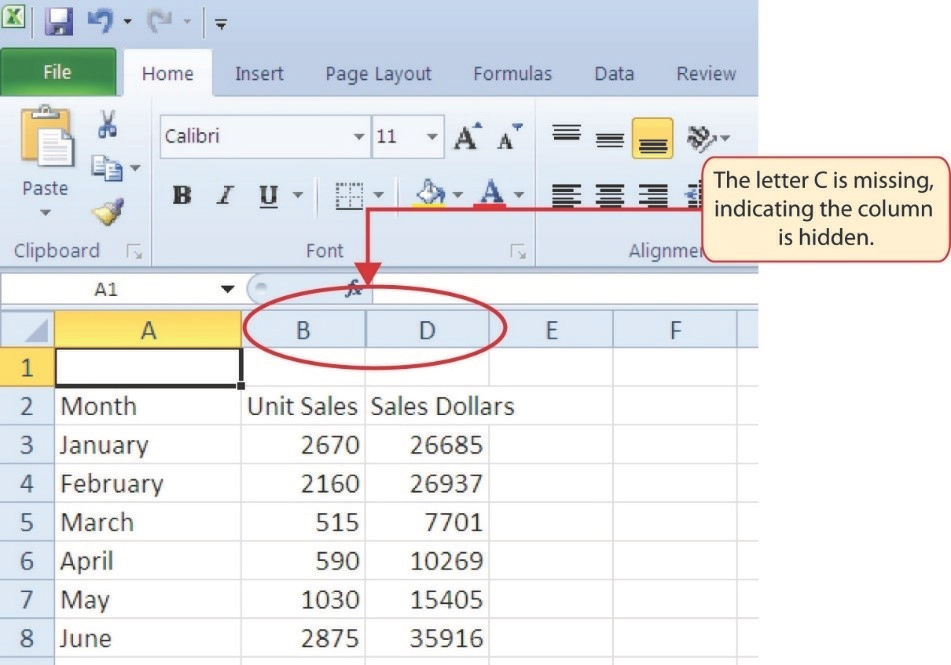
\includegraphics[width=\maxwidth{.95\linewidth}]{gfx/ch01_fig27}
	\caption{Hidden Column}
	\label{01:fig27}
\end{figure}

To unhide a column, use the following steps.

\begin{enumbox}
	\begin{enumerate}
		\item Select \fmtLoc{B1:D1} by placing the mouse pointer over cell \fmtLoc{B1}. Then left-click and drag to cell \fmtLoc{D1}.
		\item Click \fmtButton{Home $ \Rightarrow $ Cells $ \Rightarrow $ Format $ \Rightarrow $ Hide \& Unhide}. 
		\item Click the \fmtButton{Unhide Columns} option in the submenu of options. \fmtLoc{Column C} will now be visible on the worksheet.
	\end{enumerate}
\end{enumbox}

\begin{center}
	\begin{shtcutbox}{Keyboard Shortcuts}
		\textbf{Unhiding Columns}
		\\
		\begin{itemize}
			\setlength{\itemsep}{0pt}
			\setlength{\parskip}{0pt}
			\setlength{\parsep}{0pt}
			
			\item Select cells on either side of the hidden column(s).
			\item Press and hold \fmtKeystroke{Ctrl} and \fmtKeystroke{Shift} at the same time, then tap \fmtKeystroke{)}, the close parenthesis key. Note: if it does not work, then use the ribbon button.
			
		\end{itemize}
	\end{shtcutbox}
\end{center}

The following steps demonstrate how to hide rows, like hiding columns.

\begin{enumbox}
	\begin{enumerate}
		\item Click cell \fmtLoc{A3} in the \fmtWorksheet{Sheet1} worksheet.
		\item Click \fmtButton{Home $ \Rightarrow $ Cells $ \Rightarrow $ Format $ \Rightarrow $ Hide \& Unhide} to open a submenu of options.
		\item Click the \fmtButton{Hide Rows} option in the submenu of options to hide \fmtLoc{Row 3}.
	\end{enumerate}
\end{enumbox}
	
\begin{center}
	\begin{shtcutbox}{Keyboard Shortcuts}
		\textbf{Hiding Rows}
		\\
		\begin{itemize}
			\setlength{\itemsep}{0pt}
			\setlength{\parskip}{0pt}
			\setlength{\parsep}{0pt}
			
			\item Press and hold \fmtKeystroke{Ctrl}, then tap \fmtKeystroke{9}.
			
		\end{itemize}
	\end{shtcutbox}
\end{center}

To unhide a row, follow these steps.

\begin{enumbox}
	\begin{enumerate}
		\item Select \fmtLoc{A2:A4} by placing the mouse pointer over cell \fmtLoc{A2}. Then left-click and drag to cell \fmtLoc{A4}.
		\item Click \fmtButton{Home $ \Rightarrow $ Cells $ \Rightarrow $ Format $ \Rightarrow $ Hide \& Unhide} to open a submenu of options.
		\item Click the \fmtButton{Unhide Rows} option in the submenu of options to unhide \fmtLoc{Row 3}.
	\end{enumerate}
\end{enumbox}
	
\begin{center}
	\begin{shtcutbox}{Keyboard Shortcuts}
		\textbf{Unhiding Rows}
		\\
		\begin{itemize}
			\setlength{\itemsep}{0pt}
			\setlength{\parskip}{0pt}
			\setlength{\parsep}{0pt}
			
			\item Select cells above and below the hidden row(s), then press and hold \fmtKeystroke{Ctrl} and \fmtKeystroke{Shift} at the same time, then tap \fmtKeystroke{(}, the open parenthesis key.
			
		\end{itemize}
	\end{shtcutbox}
\end{center}

\begin{center}
	\begin{sklbox}{Skill Refresher}
		\textbf{Hiding Columns and Rows}
		\\
		\begin{itemize}
			\setlength{\itemsep}{0pt}
			\setlength{\parskip}{0pt}
			\setlength{\parsep}{0pt}
			
			\item Activate at least one cell in the row(s) or column(s) to be hidden.
			\item Click \textit{Home $ \Rightarrow $ Cells $ \Rightarrow $ Format $ \Rightarrow $ Hide \& Unhide}.
			\item Click either the \textit{Hide Rows} or \textit{Hide Columns} option.
			
		\end{itemize}
	\end{sklbox}
\end{center}


\begin{center}
	\begin{sklbox}{Skill Refresher}
		\textbf{Unhiding Columns and Rows}
		\\
		\begin{itemize}
			\setlength{\itemsep}{0pt}
			\setlength{\parskip}{0pt}
			\setlength{\parsep}{0pt}
			
			\item Select the cells above and below the hidden row(s) or left and right of the hidden column(s).
			\item Click \textit{Home $ \Rightarrow $ Cells $ \Rightarrow $ Format $ \Rightarrow $ Hide \& Unhide}
			\item Click either the \textit{Unhide Rows} or \textit{Unhide Columns} option.
			
		\end{itemize}
	\end{sklbox}
\end{center}

\begin{center}
	\begin{infobox}{Integrity Check}
		\textbf{Hidden Rows and Columns}
		\\
		\\
		It is common for professionals to use Excel workbooks designed by a coworker. Before using a workbook developed by someone else, always check for hidden rows and columns. It is easy to determine if a row or column is hidden by looking for missing row numbers or column letters.
	\end{infobox}
\end{center}

\subsection{Inserting Columns and Rows}

Excel workbooks others have created can be efficiently reused to eliminate creating worksheets from scratch. However, additional columns or rows may need to be added to a worksheet to accomplish a specific goal. In this case, blank columns or rows are inserted into a worksheet, as demonstrated below.

\begin{enumbox}
	\begin{enumerate}
		\item Click cell \fmtLoc{C1} in the \fmtWorksheet{Sheet1} worksheet.
		\item Click \fmtButton{Home $ \Rightarrow $ Cells $ \Rightarrow $ Insert $ \Rightarrow $ Down Arrow} (see Figure \ref{01:fig28}).
	
		\begin{figure}[H]
			\centering
			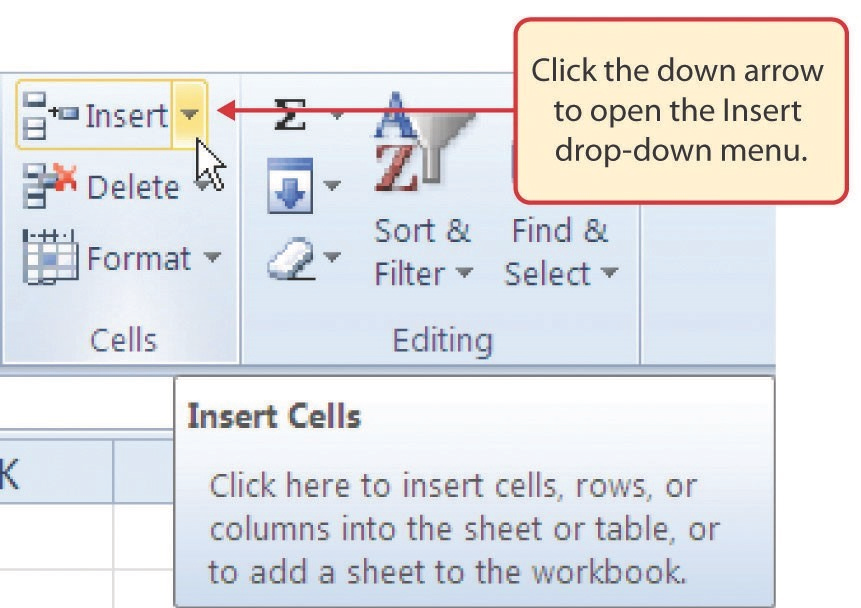
\includegraphics[width=\maxwidth{.95\linewidth}]{gfx/ch01_fig28}
			\caption{Insert Button (Down Arrow)}
			\label{01:fig28}
		\end{figure}

		\item Click the \fmtButton{Insert Sheet Columns} option from the drop-down menu (see Figure \ref{01:fig29}). A blank column will be inserted to the left of \fmtLoc{Column C}. The contents previously in \fmtLoc{Column C} now appear in \fmtLoc{Column D}. Note that columns are always inserted to the left of the activated cell.
	\end{enumerate}
\end{enumbox}

\begin{figure}[H]
	\centering
	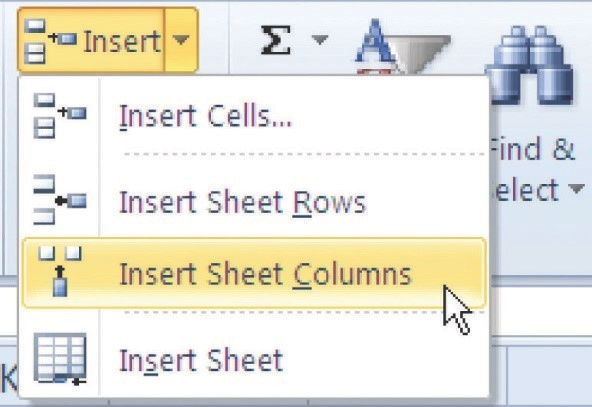
\includegraphics[width=\maxwidth{.95\linewidth}]{gfx/ch01_fig29}
	\caption{Insert Drop-Down Menu}
	\label{01:fig29}
\end{figure}

\begin{center}
	\begin{shtcutbox}{Keyboard Shortcuts}
		\textbf{Inserting Columns}
		\\
		\begin{itemize}
			\setlength{\itemsep}{0pt}
			\setlength{\parskip}{0pt}
			\setlength{\parsep}{0pt}
			
			\item Tap \fmtKeystroke{Alt} and then \fmtKeystroke{H}, \fmtKeystroke{I}, and \fmtKeystroke{C} one at a time. A column will be inserted to the left of the activated cell.
			
		\end{itemize}
	\end{shtcutbox}
\end{center}

\begin{enumbox}
	\begin{enumerate}
		\item Click cell \fmtLoc{A3} in the \fmtWorksheet{Sheet1} worksheet.
		\item Click \fmtButton{Home $ \Rightarrow $ Cells $ \Rightarrow $ Insert $ \Rightarrow $ Down Arrow} (see Figure \ref{01:fig28}).
		\item Click the \fmtButton{Insert Sheet Rows} option from the drop-down menu (see Figure \ref{01:fig29}). A blank row will be inserted above \fmtLoc{Row 3}. The contents that were previously in \fmtLoc{Row 3} now appear in \fmtLoc{Row 4}. Note that rows are always inserted above the activated cell.
	\end{enumerate}
\end{enumbox}

\begin{center}
	\begin{shtcutbox}{Keyboard Shortcuts}
		\textbf{Inserting Rows}
		\\
		\begin{itemize}
			\setlength{\itemsep}{0pt}
			\setlength{\parskip}{0pt}
			\setlength{\parsep}{0pt}
			
			\item Tap \fmtKeystroke{Alt}, and then tap \fmtKeystroke{H}, \fmtKeystroke{I}, and \fmtKeystroke{R} one at a time. A row will be inserted above the activated cell.
			
		\end{itemize}
	\end{shtcutbox}
\end{center}

\begin{center}
	\begin{sklbox}{Skill Refresher}
		\textbf{Inserting Columns and Rows}
		\\
		\begin{itemize}
			\setlength{\itemsep}{0pt}
			\setlength{\parskip}{0pt}
			\setlength{\parsep}{0pt}
			
			\item Activate the cell to the right of the desired blank column or below the desired blank row.
			\item Click \textit{Home $ \Rightarrow $ Cells $ \Rightarrow $ Insert $ \Rightarrow $ Down Arrow}
			\item Click either the \textit{Insert Sheet Columns} or \textit{Insert Sheet Rows} option.
			
		\end{itemize}
	\end{sklbox}
\end{center}

\subsection{Moving Data}

Once data is entered into a worksheet, it can be moved to different locations, as demonstrated below.

\begin{enumbox}
	\begin{enumerate}
		\item Select \fmtLoc{D2:D15} by placing the mouse pointer over cell \fmtLoc{D2}. Then left-click and drag to cell \fmtLoc{D15}.
		\item Bring the mouse pointer to the left edge of cell \fmtLoc{D2}. Notice that the white block plus sign changes to cross arrows (see Figure \ref{01:fig30}), indicating the data can be dragged to a new location by left-clicking the mouse.
	
		\begin{figure}[H]
			\centering
			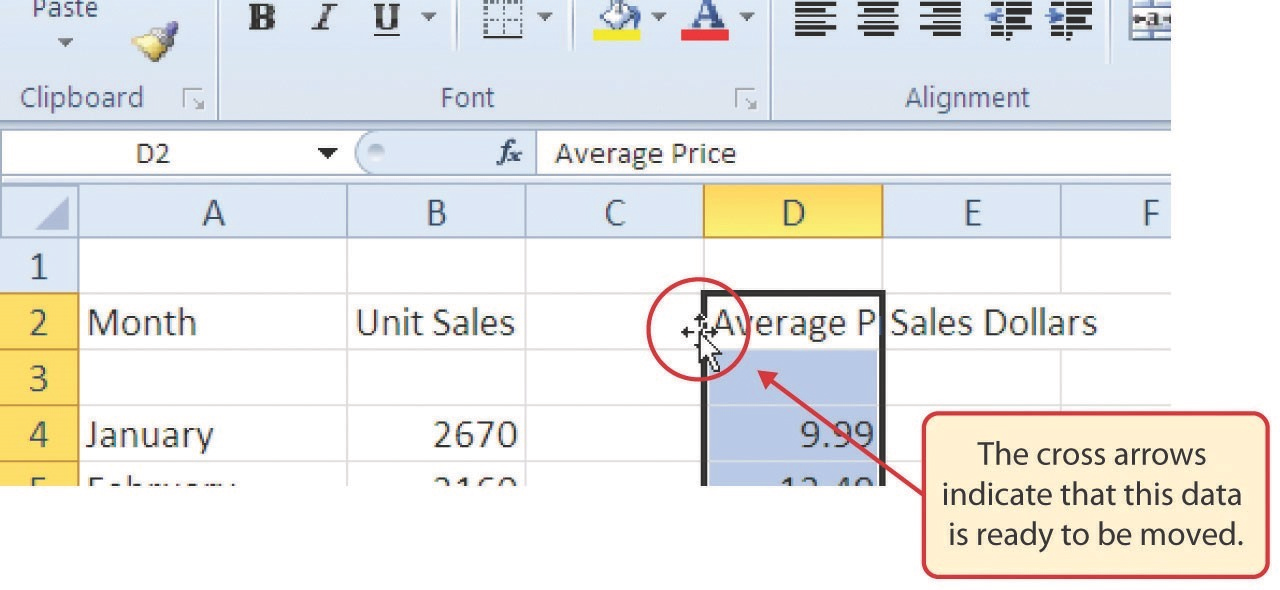
\includegraphics[width=\maxwidth{.95\linewidth}]{gfx/ch01_fig30}
			\caption{Moving Data}
			\label{01:fig30}
		\end{figure}

		\item Left-click and drag the mouse pointer to cell \fmtLoc{C2}.
		\item Release the left mouse button. The data now appears in \fmtLoc{Column C}.
		\item Click the \textit{Undo} button in the \fmtButton{Quick Access Toolbar} to move the data back to \fmtLoc{Column D}.
	\end{enumerate}
\end{enumbox}

\begin{center}
	\begin{infobox}{Integrity Check}
		\textbf{Moving Data}
		\\
		\\
		Before moving data on a worksheet, identify all the components that belong to the moving series. For example, if a column of data is being moved, make sure the column heading is included. Also, ensure all values are selected in the column before moving it.
	\end{infobox}
\end{center}


\subsection{Deleting Columns and Rows}

Occasionally, it may be necessary to delete entire columns or rows of data from a worksheet. For example, a worksheet may contain blank columns or rows that need to be removed. The methods for removing cell contents were covered earlier and can be used to delete unwanted data. However, to delete an entire column or row in a workbook, use the following steps.

\begin{enumbox}
	\begin{enumerate}
		\item Click cell \fmtLoc{A3}.
		\item Click \fmtButton{Home $ \Rightarrow $ Cells $ \Rightarrow $ Delete $ \Rightarrow $ Down Arrow}
		\item Click the \fmtButton{Delete Sheet Rows} option from the drop-down menu (see Figure \ref{01:fig31}) to remove \fmtLoc{Row 3} and shift everything up one row.
	\end{enumerate}
\end{enumbox}
	
\begin{figure}[H]
	\centering
	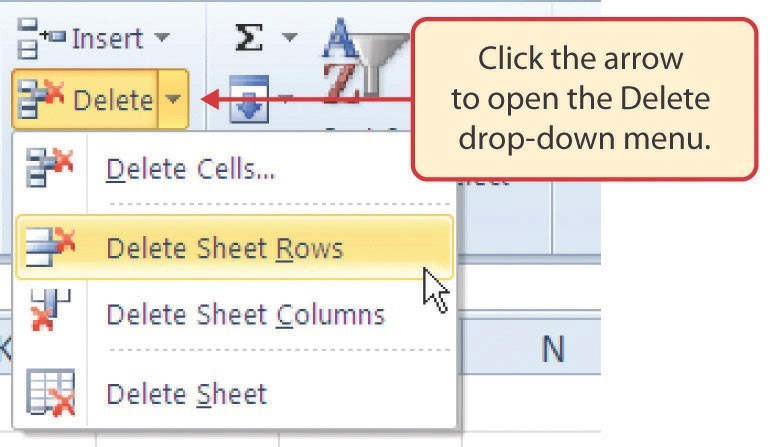
\includegraphics[width=\maxwidth{.95\linewidth}]{gfx/ch01_fig31}
	\caption{Delete Drop-Down Menu}
	\label{01:fig31}
\end{figure}

\begin{center}
	\begin{shtcutbox}{Keyboard Shortcuts}
		\textbf{Deleting Rows}
		\\
		\begin{itemize}
			\setlength{\itemsep}{0pt}
			\setlength{\parskip}{0pt}
			\setlength{\parsep}{0pt}
			
			\item Tap \fmtKeystroke{Alt}, and then \fmtKeystroke{H}, \fmtKeystroke{D}, and \fmtKeystroke{R} one at a time. The row with the activated cell will be deleted.
			
		\end{itemize}
	\end{shtcutbox}
\end{center}

\begin{enumbox}
	\begin{enumerate}
		\item Click cell \fmtLoc{C1}.
		\item Click \fmtButton{Home $ \Rightarrow $ Cells $ \Rightarrow $ Delete $ \Rightarrow $ Down Arrow}.
		\item Click the \fmtButton{Delete Sheet Columns} option from the drop-down menu (see Figure \ref{01:fig31}) to remove \fmtLoc{Column C} and shift everything one column to the left.
		\item Save the changes to the workbook by clicking either \fmtButton{Quick Access Toolbar $ \Rightarrow $ Save} or \fmtButton{File $ \Rightarrow $ Save}.
	\end{enumerate}
\end{enumbox}

\begin{center}
	\begin{shtcutbox}{Keyboard Shortcuts}
		\textbf{Deleting Columns}
		\\
		\begin{itemize}
			\setlength{\itemsep}{0pt}
			\setlength{\parskip}{0pt}
			\setlength{\parsep}{0pt}
			
			\item Tap \fmtKeystroke{Alt} and then \fmtKeystroke{H}, \fmtKeystroke{D}, and \fmtKeystroke{C} one at a time. The column with the activated cell will be deleted.
			
		\end{itemize}
	\end{shtcutbox}
\end{center}

\begin{center}
	\begin{sklbox}{Skill Refresher}
		\textbf{Deleting Columns and Rows}
		\\
		\begin{itemize}
			\setlength{\itemsep}{0pt}
			\setlength{\parskip}{0pt}
			\setlength{\parsep}{0pt}
			
			\item Activate any cell in the row or column that is to be deleted.
			\item Click \textit{Home $ \Rightarrow $ Cells $ \Rightarrow $ Delete $ \Rightarrow $ Down Arrow}.
			\item Click either \textit{Delete Sheet Columns} or \textit{Delete Sheet Rows}.
			
		\end{itemize}
	\end{sklbox}
\end{center}

\begin{center}
	\begin{tkwbox}{Key Take-Aways}
		\textbf{Entering, Editing, and Managing Data}
		\\
		\begin{itemize}
			\setlength{\itemsep}{0pt}
			\setlength{\parskip}{0pt}
			\setlength{\parsep}{0pt}
			
			\item Column headings should be used in a worksheet and should accurately describe the data contained in each column.
			\item Using symbols such as dollar signs when entering numbers into a worksheet can slow down the data entry process.
			\item Worksheets must be carefully proofread when data has been manually entered.
			\item The Undo command is a valuable tool for recovering data deleted from a worksheet.
			\item When using a worksheet developed by someone else, look carefully for hidden columns or rows.
			
		\end{itemize}
	\end{tkwbox}
\end{center}

\section{Formatting and Data Analysis}

\begin{center}
	\begin{objbox}{Learning Objectives}
		\begin{itemize}
			\setlength{\itemsep}{0pt}
			\setlength{\parskip}{0pt}
			\setlength{\parsep}{0pt}
			
			\item Use formatting techniques as introduced in the \textit{Excel Spreadsheet Guidelines} below to enhance the appearance of a worksheet.
			\item Understand how to align data in cell locations.
			\item Examine how to enter multiple lines of text in a cell location.
			\item Understand how to add borders to a worksheet.
			\item Examine how to use the AutoSum feature to calculate totals.
			\item Use the Cut, Copy, and Paste commands to manipulate the data on a worksheet.
			\item Understand how to move, rename, insert, and delete worksheet tabs.
		\end{itemize}
	\end{objbox}
\end{center}

This section addresses formatting commands used to enhance a worksheet's visual appearance. It also introduces mathematical calculations. The skills introduced in this section provide powerful tools for analyzing the data used in this workbook. They will highlight how Excel makes critical decisions in virtually any career. Additionally, \textit{Excel Spreadsheet Guidelines} for format and appearance will be introduced as a format to be used for the spreadsheets submitted as part of this course.

\subsection{Formatting Data and Cells}

Enhancing a worksheet's visual appearance is a critical step when creating a tool to help coworkers make decisions. For example, professional formatting standards are used when worksheets contain only currency data. The following \textit{Excel Guidelines for Formatting} will be used for this course. Figure \ref{01:fig32} displays how to format a column when all numbers are currency. Only the first row of the data and the totals should be formatted with Excel's \textit{Accounting} format, while the other numbers are formatted with the \textit{Comma} style. There also needs to be a top border above the numbers in the total row. If any numbers have cents, format them all with two decimal places; otherwise, use zero decimal places.

\begin{figure}[H]
	\centering
	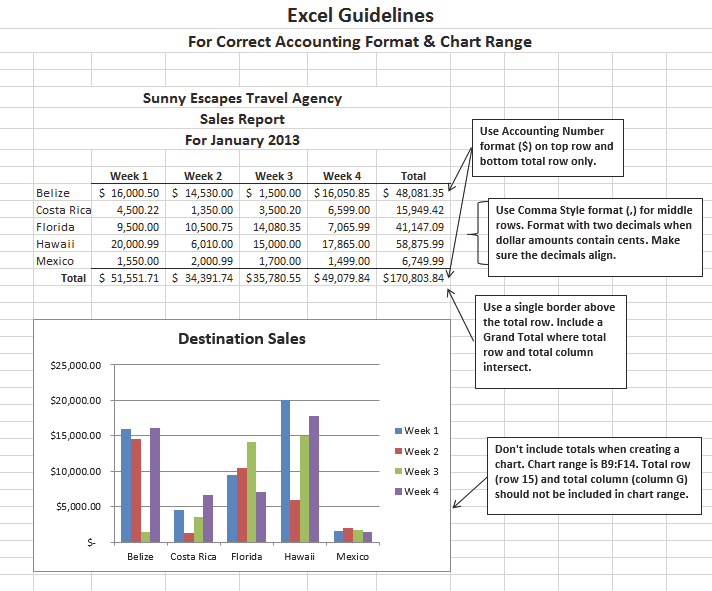
\includegraphics[width=\maxwidth{.95\linewidth}]{gfx/ch01_fig32}
	\caption{Excel Guidelines for Formatting Currency}
	\label{01:fig32}
\end{figure}

Often, an Excel worksheet contains values that are both currency and non-currency in nature. When that is the case, use the guidelines in Figure \ref{01:fig33}.

\begin{figure}[H]
	\centering
	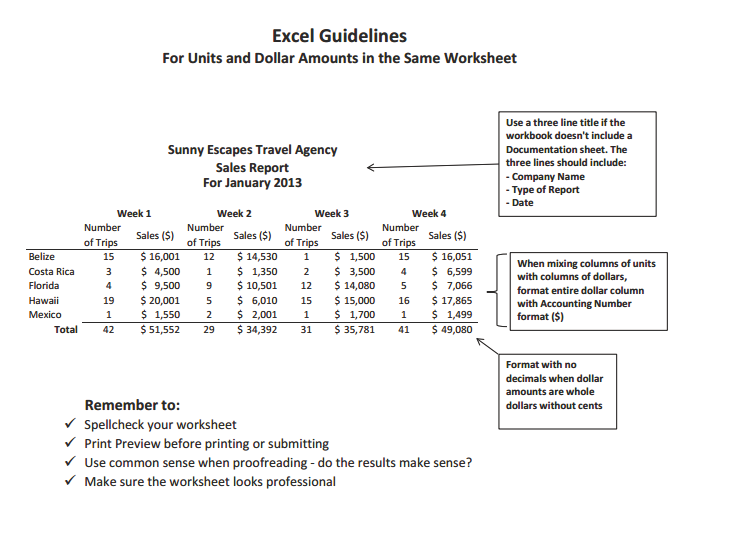
\includegraphics[width=\maxwidth{.95\linewidth}]{gfx/ch01_fig33}
	\caption{Excel Guidelines for Formatting Numbers}
	\label{01:fig33}
\end{figure}

The following steps demonstrate several fundamental formatting skills that will be applied to the workbook developed for this chapter. Several of these formatting skills are identical to ones used in other Microsoft applications such as Microsoft\textsuperscript{\textregistered} Word\textsuperscript{\textregistered} or  PowerPoint\textsuperscript{\textregistered}.

\begin{enumbox}
	\begin{enumerate}
		\item Select \fmtLoc{A2:D2} by placing the mouse pointer over cell \fmtLoc{A2} in \fmtWorksheet{Sheet1}. Then left-click and drag to cell \fmtLoc{D2}. 
		\item Click \fmtButton{Home $ \Rightarrow $ Font $ \Rightarrow $ Bold} (see Figure \ref{01:fig34}).
		\item Click \fmtButton{Home $ \Rightarrow $ Font $ \Rightarrow $ Border $ \Rightarrow $ Down Arrow}. Select the \fmtButton{Bottom Border} option from the list to place a border on the bottom of \fmtLoc{Row 2}.
	\end{enumerate}
\end{enumbox}

\begin{figure}[H]
	\centering
	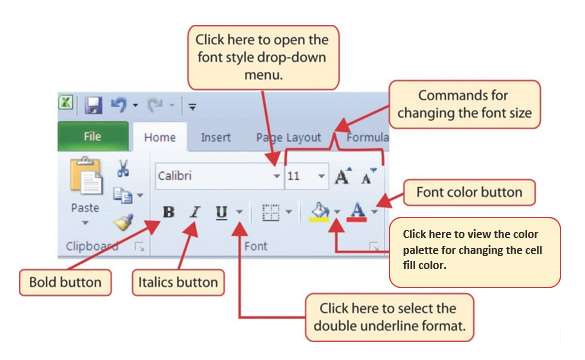
\includegraphics[width=\maxwidth{.95\linewidth}]{gfx/ch01_fig34}
	\caption{The Font Command Group}
	\label{01:fig34}
\end{figure}

\begin{center}
	\begin{shtcutbox}{Keyboard Shortcuts}
		\textbf{Text Formats}
		\\
		\begin{itemize}
			\setlength{\itemsep}{0pt}
			\setlength{\parskip}{0pt}
			\setlength{\parsep}{0pt}
			
			\item Bold: press and hold \fmtKeystroke{Ctrl}, then tap \fmtKeystroke{B}.
			\item Italics: press and hold \fmtKeystroke{Ctrl}, then tap \fmtKeystroke{I}.
			\item Underline: press and hold \fmtKeystroke{Ctrl}, then tap \fmtKeystroke{U}.
			
		\end{itemize}
	\end{shtcutbox}
\end{center}

\begin{enumbox}
	\begin{enumerate}
		\item Select \fmtLoc{A15:D15} by placing the mouse pointer over cell \fmtLoc{A15}. Then left-click and drag to cell \fmtLoc{D15}.
		\item Click \fmtButton{Home $ \Rightarrow $ Font $ \Rightarrow $ Bold}.
		\item Click \fmtButton{Home $ \Rightarrow $ Font $ \Rightarrow $ Border $ \Rightarrow $ Down Arrow}. Select the \fmtButton{Top Border} option from the list to place a border on the top of \fmtLoc{Row 15}, where totals will eventually be displayed.
		\item Select \fmtLoc{B3:B14} by placing the mouse pointer over cell \fmtLoc{B3}. Then left-click and drag to cell \fmtLoc{B14}.
		\item Click \fmtButton{Home $ \Rightarrow $ Number $ \Rightarrow $ Comma Style}. This feature adds a comma and two decimal places to numbers in the cell (see Figure \ref{01:fig35}).
	\end{enumerate}
\end{enumbox}

\begin{figure}[H]
	\centering
	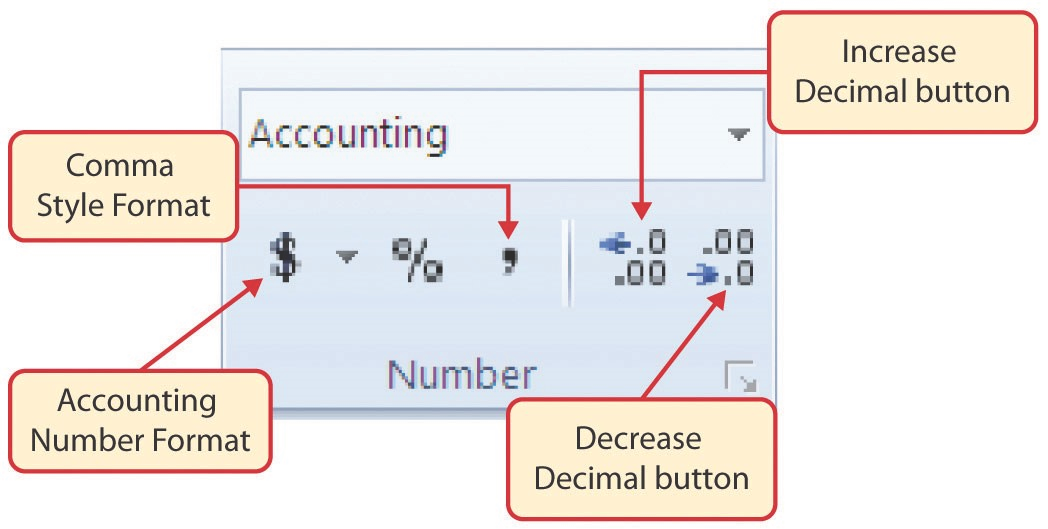
\includegraphics[width=\maxwidth{.95\linewidth}]{gfx/ch01_fig35}
	\caption{The Number Command Group}
	\label{01:fig35}
\end{figure}

\begin{center}
	\begin{infobox}{Why?}
		\textbf{Format Column Headings and Totals}
		\\
		\\
		Applying formatting enhancements to the column headings and column totals in a worksheet is an important technique, especially if the workbook is shared with others. These formatting techniques allow users of the worksheet to see the column headings that define the data. In addition, the column totals usually contain essential data on a worksheet concerning making decisions, and formatting techniques allow users to find this information quickly.
	\end{infobox}
\end{center}

\begin{enumbox}
	\begin{enumerate}
		\item Since the figures in this range do not include cents, click \fmtButton{Home $ \Rightarrow $ Number $ \Rightarrow $ Decrease Decimal} two times (see Figure \ref{01:fig35}).
		\item The numbers will be reduced to zero decimal places.
		\item Select \fmtLoc{C3:C14} by placing the mouse pointer over cell \fmtLoc{C3}, then left-clicking and dragging to cell \fmtLoc{C14}.
		\item Click \fmtButton{Home $ \Rightarrow $ Number $ \Rightarrow $ Accounting Number} (see Figure \ref{01:fig35}) to add a currency symbol and two decimal places to the values. Use the \textit{Accounting} format on all values in this range since the worksheet contains non-currency and currency data.
		\item Select \fmtLoc{D3:D14} by placing the mouse pointer over \fmtLoc{D3}, then left-clicking and dragging to \fmtLoc{D14}.
		\item Apply the \textit{Accounting} number format to add the US currency symbol to the values and set them to two decimal places.
		\item Click \fmtButton{Home $ \Rightarrow $ Number $ \Rightarrow $ Decrease Decimal} two times to reduce the decimal places to zero since there are no cents in these figures.
		\item Select \fmtLoc{A1:D1} by placing the mouse pointer over cell \fmtLoc{A1} then left-clicking and dragging over to cell \fmtLoc{D1}.
		\item Click \fmtButton{Home $ \Rightarrow $ Font $ \Rightarrow $ Fill Color $ \Rightarrow $ Down Arrow} (see Figure \ref{01:fig36}) to prepare the range for a worksheet title.

		\begin{figure}[H]
			\centering
			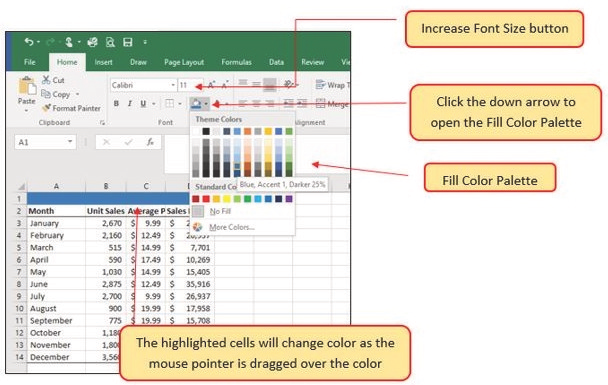
\includegraphics[width=\maxwidth{.95\linewidth}]{gfx/ch01_fig36}
			\caption{Fill Color Palette}
			\label{01:fig36}
		\end{figure}

		\item Click the \textit{Blue, Accent 1, Darker 25\%} color from the palette (see Figure \ref{01:fig36}). Notice that as the mouse pointer moves over the color palette, a preview of the color appears in the selected cells. That makes it easy to experiment with various colors.
		\item Click on \fmtLoc{A1} and enter \fmtTyping{General Merchandise World} as the worksheet title.
		\item Click on \fmtLoc{A2} and then click on \fmtLoc{A1} to select the cell that contains the text rather than the text itself.
		\item Since the black font is difficult to read on the blue background, change the font color to be more visible. Click \fmtButton{Home $ \Rightarrow $ Font $ \Rightarrow $ Font Color $ \Rightarrow $ Down Arrow} and select \textit{White} as the font color for this range (see Figure \ref{01:fig34}).
		\item Select \fmtLoc{A1:D15} by placing the mouse pointer over cell \fmtLoc{A1}. Then left-click and drag to cell \fmtLoc{D15}.
		\item Click \fmtButton{Home $ \Rightarrow $ Font $ \Rightarrow $ Down Arrow} and select \textit{Arial} as the font for this range (see Figure \ref{01:fig34}). Notice that as the mouse pointer moves over the font style options, it changes the selected cells to make previewing various font options easy.
		\item Expand the column width of \fmtLoc{Column D} to $ 14 $ characters.
	\end{enumerate}
\end{enumbox}

Figure \ref{01:fig37} shows how the \fmtWorksheet{Sheet1} worksheet should appear after applying the formatting techniques.

\begin{figure}[H]
	\centering
	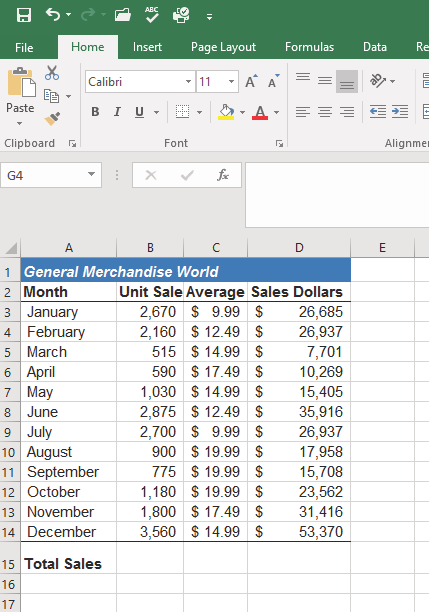
\includegraphics[width=\maxwidth{.95\linewidth}]{gfx/ch01_fig37}
	\caption{Formatting Techniques Applied}
	\label{01:fig37}
\end{figure}

\begin{center}
	\begin{infobox}{Why}
		\textbf{Hashtags (\#\#\#\#) Appear in Columns}
		\\
		\\
		When a column is too narrow for a long number, Excel will automatically convert the number to a series of hashtags (\#\#\#\#). In the case of words or text data, Excel will only show the characters that fit in the column; but truncated numeric data can appear much smaller than the actual cell contents. To remove the hashtags, increase the width of the column.
	\end{infobox}
\end{center}

\begin{center}
	\begin{infobox}{Why}
		\textbf{Hashtags (\#\#\#\#) Appear in Columns}
		\\
		\\
		When a column is too narrow for a long number, Excel will automatically convert the number to a series of hashtags (\#\#\#\#). In the case of words or text data, Excel will only show the characters that fit in the column. However, long numbers are not truncated but are indicated with the hashtags. To remove the hashtags, increase the width of the column.
	\end{infobox}
\end{center}


\subsection{Data Alignment (Wrap Text, Merge Cells, and Center)}

The skills presented in this section show how data is aligned within cell locations. For example, text and numbers can be centered, left-aligned, and right-aligned in a cell. In some cases, multi-word text entries may need to be stacked vertically instead of expanding the width of a column, referred to as wrapping text. These skills are demonstrated in the following steps.

\begin{enumbox}
	\begin{enumerate}
		\item Select \fmtLoc{B2:D2} by placing the mouse pointer over cell \fmtLoc{B2}. Then left-click and drag to cell \fmtLoc{D2}.
		\item Click \fmtButton{Home $ \Rightarrow $ Alignment $ \Rightarrow $ Center} (see Figure \ref{01:fig38}) to center the column headings in each cell location. Notice the difference between text that is centered horizontally and text that is middle aligned vertically.
		
		\begin{figure}[H]
			\centering
			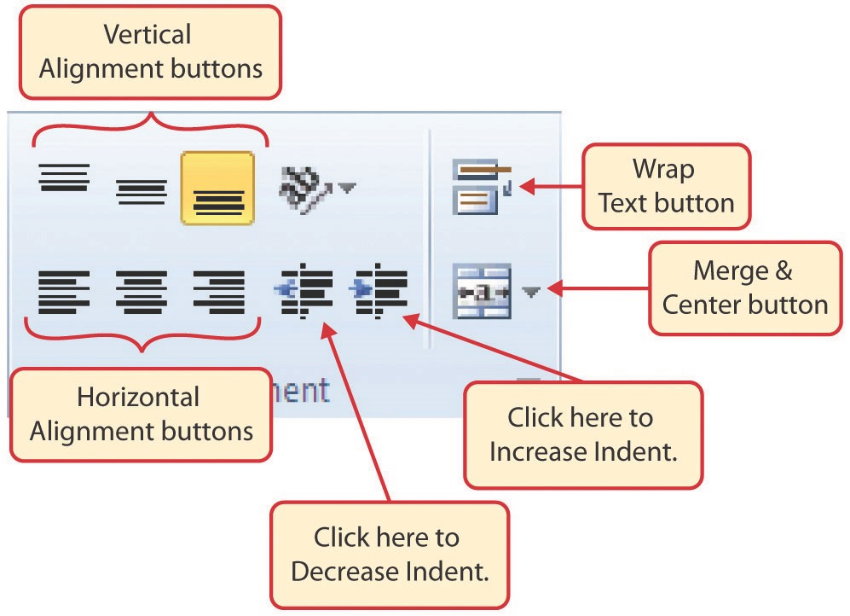
\includegraphics[width=\maxwidth{.95\linewidth}]{gfx/ch01_fig38}
			\caption{Alignment Group in Home Tab}
			\label{01:fig38}
		\end{figure}
		
		\item Click \fmtButton{Home $ \Rightarrow $ Alignment $ \Rightarrow $ Wrap Text} (see Figure \ref{01:fig38}). The height of \fmtLoc{Row 2} automatically expands, and the words that were cut off because the columns were too narrow are now stacked vertically.
		\item Select \fmtLoc{A1:D1} by placing the mouse pointer over cell \fmtLoc{A1}. Then left-click and drag to cell \fmtLoc{D1}.
		\item Click \fmtButton{Home $ \Rightarrow $ Alignment $ \Rightarrow $ Merge \& Center $ \Rightarrow $ Down Arrow}.
		\item Click the \fmtButton{Merge \& Center} option (see Figure \ref{01:fig39}) to create one prominent cell across the top of the data set.
	\end{enumerate}
\end{enumbox}

\begin{figure}[H]
	\centering
	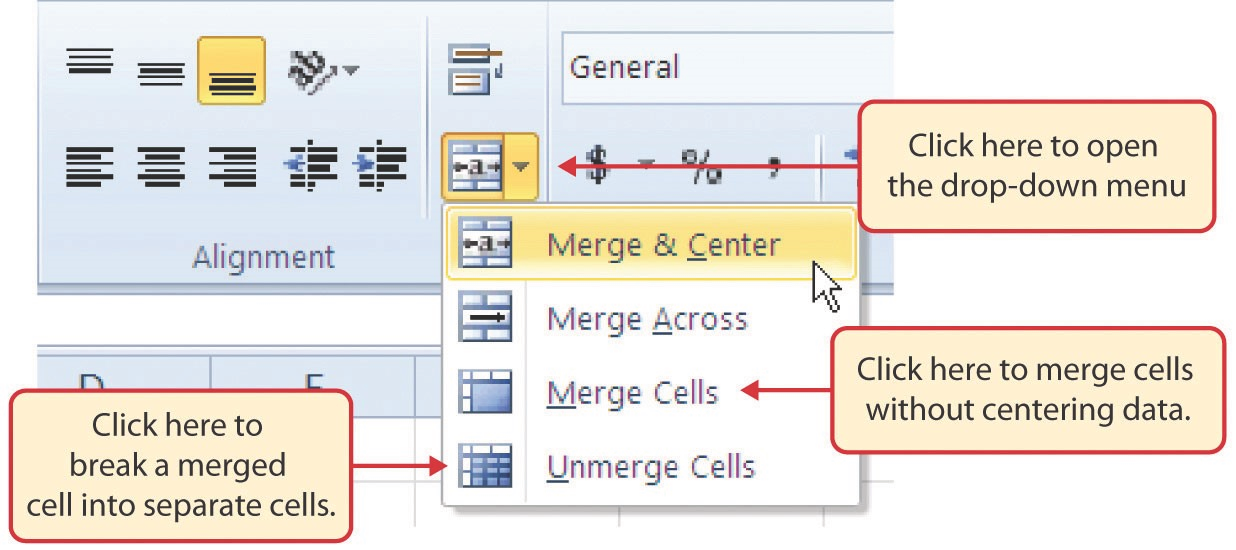
\includegraphics[width=\maxwidth{.95\linewidth}]{gfx/ch01_fig39}
	\caption{Merge Cell Drop-Down Menu}
	\label{01:fig39}
\end{figure}

\begin{center}
	\begin{shtcutbox}{Keyboard Shortcuts}
		\textbf{Merge Commands}
		\\
		\begin{itemize}
			\setlength{\itemsep}{0pt}
			\setlength{\parskip}{0pt}
			\setlength{\parsep}{0pt}
			
			\item \textbf{Wrap Text}: Tap \fmtKeystroke{Alt} and then \fmtKeystroke{H} and \fmtKeystroke{W} one at a time.
			\item \textbf{Merge \& Center}: Tap \fmtKeystroke{Alt} and then \fmtKeystroke{H}, \fmtKeystroke{M}, and \fmtKeystroke{C} one at a time.
			\item \textbf{Merge Cells}: Tap \fmtKeystroke{Alt} and then \fmtKeystroke{H}, \fmtKeystroke{M}, and \fmtKeystroke{M} one at a time.
			\item \textbf{Unmerge Cells}: Tap \fmtKeystroke{Alt} and then \fmtKeystroke{H}, \fmtKeystroke{M}, and \fmtKeystroke{U} one at a time.
			
		\end{itemize}
	\end{shtcutbox}
\end{center}

\begin{center}
	\begin{infobox}{Why?}
		\textbf{Wrap Text}
		\\
		\\
		Wrapped text significantly reduces the need to expand the column width to accommodate multi-word column headings. Wide columns reduce the amount of data that can fit on a printed piece of paper or one screen, so analyzing data becomes cumbersome.
	\end{infobox}
\end{center}

Figure \ref{01:fig40} shows the \textit{Sheet1} worksheet with the applied data alignment commands. The following section will clarify the reason for merging cells $ A1 $:$ D1 $.

\begin{figure}[H]
	\centering
	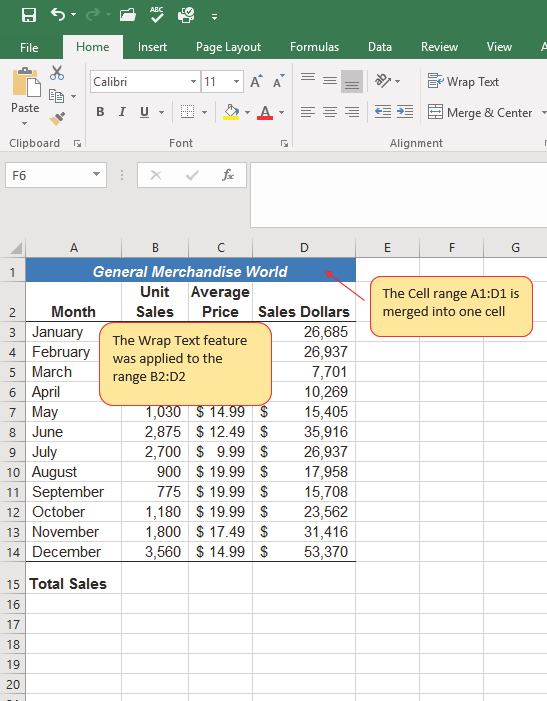
\includegraphics[width=\maxwidth{.95\linewidth}]{gfx/ch01_fig40}
	\caption{Sheet1 with Data Alignment Features Added}
	\label{01:fig40}
\end{figure}

\begin{center}
	\begin{infobox}{Why?}
		\textbf{Merge \& Center}
		\\
		\\
		One of the most common reasons the \fmtButton{Merge \& Center} command is used is to center the worksheet's title directly above the columns of data. Once the cells above the column headings are merged, a title can be centered above the columns of data. It is challenging to center the title over the columns of data if the cells are not merged.
	\end{infobox}
\end{center}

\begin{center}
	\begin{sklbox}{Skill Refresher}
		\textbf{Wrap Text}
		\\
		\begin{itemize}
			\setlength{\itemsep}{0pt}
			\setlength{\parskip}{0pt}
			\setlength{\parsep}{0pt}
			
			\item Activate the cell or range of cells that contain text data.
			\item Click \textit{Home $ \Rightarrow $ Alignment $ \Rightarrow $ Wrap Text}.
			
		\end{itemize}
	\end{sklbox}
\end{center}

\begin{center}
	\begin{sklbox}{Skill Refresher}
		\textbf{Merge Cells}
		\\
		\begin{itemize}
			\setlength{\itemsep}{0pt}
			\setlength{\parskip}{0pt}
			\setlength{\parsep}{0pt}
			
			\item Select a range of cells that will be merged.
			\item Click \textit{Home $ \Rightarrow $ Alignment $ \Rightarrow $ Merge \& Center Down Arrow}.
			\item Select an option from the \textit{Merge \& Center} list.
			
		\end{itemize}
	\end{sklbox}
\end{center}

\subsection{Entering Multiple Lines of Text}

In the \textit{Sheet1} worksheet, the cells in $ A1 $:$ D1 $ were merged to add a title to the worksheet. This worksheet will contain both a title and a subtitle. The following steps explain how to enter text into a cell and determine where the second line of text should begin.

\begin{enumbox}
	\begin{enumerate}
		\item Click cell \fmtLoc{A1} in the \fmtWorksheet{Sheet1} worksheet. Since the cells were merged, clicking cell \fmtLoc{A1} will automatically activate \fmtLoc{A1:D1}. Position the mouse to the end of the title, directly after the ``d'' in the word ``World,'' and double-click to get a cursor (flashing I-beam).
		\item Press and hold \fmtKeystroke{Alt}, then tap \fmtKeystroke{Enter} to start a new line of text in this cell location.
		\item Type the text \fmtTyping{Retail Sales (in millions)}, then tap \fmtKeystroke{Enter}.
		\item Click cell \fmtLoc{A1}. 
		\item Increase the height of Row $ 1 $ to $ 30 $ points. Once the row height increases, all the text typed into the cell will be visible (see Figure \ref{01:fig41}).
		\item Click \fmtButton{Home $ \Rightarrow $ Font $ \Rightarrow $ Bold}.
		\item Click \fmtButton{Home $ \Rightarrow $ Font $ \Rightarrow $ Italics}.
	\end{enumerate}
\end{enumbox}

\begin{figure}[H]
	\centering
	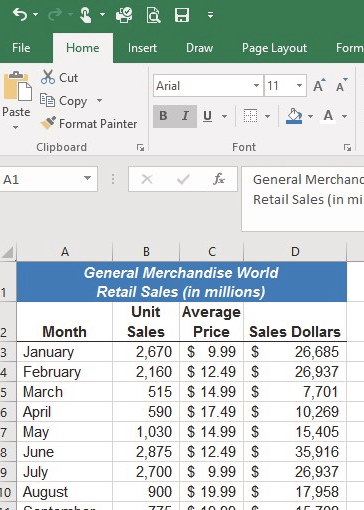
\includegraphics[width=\maxwidth{.95\linewidth}]{gfx/ch01_fig41}
	\caption{Title \& Subtitle Added to the Worksheet}
	\label{01:fig41}
\end{figure}

\begin{center}
	\begin{sklbox}{Skill Refresher}
		\textbf{Entering Multiple Lines of Text}
		\\
		\begin{itemize}
			\setlength{\itemsep}{0pt}
			\setlength{\parskip}{0pt}
			\setlength{\parsep}{0pt}
			
			\item Activate a cell location.
			\item Type the first line of text.
			\item Press and hold \fmtKeystroke{Alt}, then tap \fmtKeystroke{Enter}.
			\item Type the second line of text and tap \fmtKeystroke{Enter}.
			
		\end{itemize}
	\end{sklbox}
\end{center}

\subsection{Borders (Adding Lines to a Worksheet)}

In Excel, adding custom lines to a worksheet is known as adding borders. Borders are different from the worksheet's gridlines since they define perimeters around a cell range. Borders add a variety of line styles to a worksheet, making it easier to understand. The following steps illustrate methods for adding preset and custom borders to a worksheet.

\begin{enumbox}
	\begin{enumerate}
		\item Click \fmtButton{Home $ \Rightarrow $ Font $ \Rightarrow $ Borders $ \Rightarrow $ Down Arrow} to view border options (see Figure \ref{01:fig42}).

		\begin{figure}[H]
			\centering
			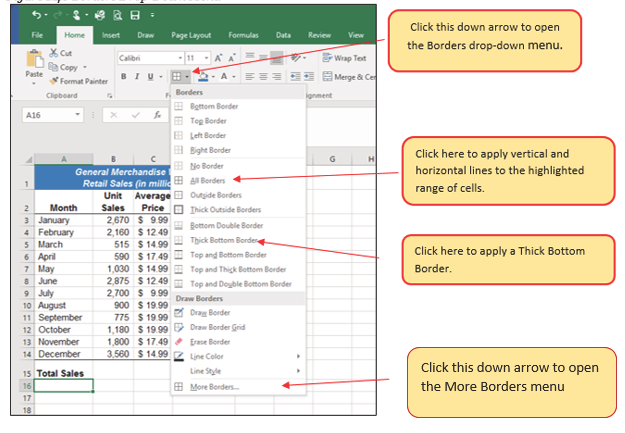
\includegraphics[width=\maxwidth{.95\linewidth}]{gfx/ch01_fig42}
			\caption{Borders Drop-Down Menu}
			\label{01:fig42}
		\end{figure}

		\item Select \fmtLoc{A1:D15} by placing the mouse pointer over cell \fmtLoc{A1}. Then left-click and drag to cell \fmtLoc{D15}. 
		\item Click \fmtButton{Home $ \Rightarrow $ Font $ \Rightarrow $ Borders $ \Rightarrow $ Down Arrow $ \Rightarrow $ All Borders} (see Figure \ref{01:fig42}) to add vertical and horizontal lines to \fmtLoc{A1:D15}.
		\item Select \fmtLoc{A2:D2} by placing the mouse pointer over cell \fmtLoc{A2}. Then left-click and drag to cell \fmtLoc{D2}.
		\item Click \fmtButton{Home $ \Rightarrow $ Font $ \Rightarrow $ Borders $ \Rightarrow $ Down Arrow $ \Rightarrow $ Thick Bottom Border}
		\item Select \fmtLoc{A14:D14} by placing the mouse pointer over cell \fmtLoc{A14}. Then left-click and drag to cell \fmtLoc{D14}.
		\item Click \fmtButton{Home $ \Rightarrow $ Font $ \Rightarrow $ Borders $ \Rightarrow $ Down Arrow $ \Rightarrow $ Thick Bottom Border}. The thick border will help maintain the \textit{Excel Formatting Guidelines}.
		\item Select \fmtLoc{A1:D15}.
		\item Click \fmtButton{Home $ \Rightarrow $ Font $ \Rightarrow $ Borders $ \Rightarrow $ Down Arrow $ \Rightarrow $ More Borders...} to open the \textit{Format Cells} dialog box (see Figure \ref{01:fig43}). All Excel formatting commands can be accessed through this dialog box.
		\item In the \textit{Style} section of the \textit{Borders} tab, click the thickest line style (see Figure \ref{01:fig43}).
		\item Click the \fmtButton{Outline} button in the \textit{Presets} section (see Figure \ref{01:fig43}).
		\item Click the \fmtButton{OK} button at the bottom of the dialog box (see Figure \ref{01:fig43}).
	\end{enumerate}
\end{enumbox}
	
\begin{figure}[H]
	\centering
	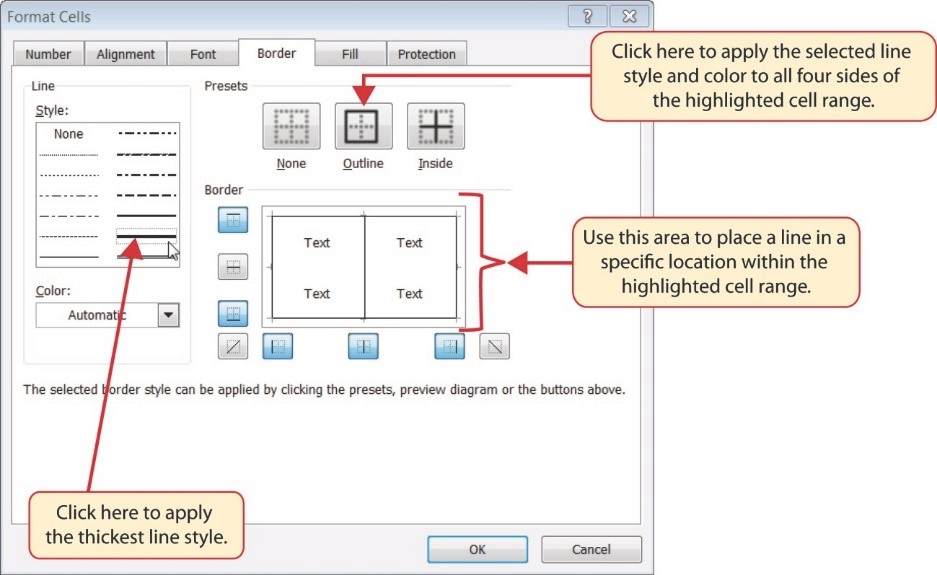
\includegraphics[width=\maxwidth{.95\linewidth}]{gfx/ch01_fig43}
	\caption{Borders Tab of the Format Cells Dialog Box}
	\label{01:fig43}
\end{figure}

The \textit{Sheet1} worksheet should now look like Figure \ref{01:fig44}.

\begin{figure}[H]
	\centering
	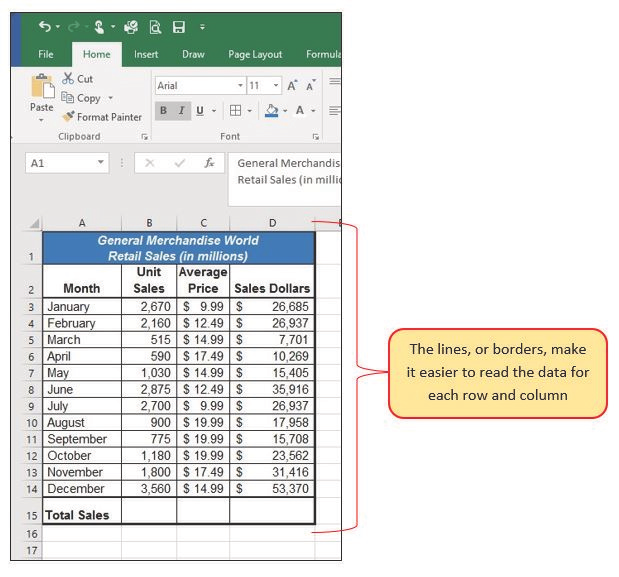
\includegraphics[width=\maxwidth{.95\linewidth}]{gfx/ch01_fig44}
	\caption{Borders Added to the Sheet1 Worksheet}
	\label{01:fig44}
\end{figure}

\begin{center}
	\begin{sklbox}{Skill Refresher}
		\textbf{Preset Borders}
		\\
		\begin{itemize}
			\setlength{\itemsep}{0pt}
			\setlength{\parskip}{0pt}
			\setlength{\parsep}{0pt}
			
			\item Select a range of cells that require borders.
			\item Click the \textit{Home} tab of the Ribbon.
			\item Click the down arrow next to the \textit{Borders} button.
			\item Select an option from the preset borders list.
			
		\end{itemize}

		\hfill \break
		\textbf{Custom Borders}
		\\
		\begin{itemize}
			\setlength{\itemsep}{0pt}
			\setlength{\parskip}{0pt}
			\setlength{\parsep}{0pt}
			
			\item Select a range of cells that require borders.
			\item Click \textit{Home $ \Rightarrow $ Font $ \Rightarrow $ Borders $ \Rightarrow $ Down Arrow $ \Rightarrow $ More Borders...}
			\item Select a line style and line color.
			\item Select a placement option.
			\item Click the \textit{OK} button on the dialog box.
			
		\end{itemize}

	\end{sklbox}
\end{center}

\subsection{AutoSum}

Notice \textit{Row 15} in Figure \ref{01:fig44} shows column totals. Applying mathematical computations to a range of cells is accomplished through functions in Excel\footnote{Chapter \ref{ch03:formulas}, \nameref{ch03:formulas}, page \pageref{ch03:formulas}, reviews mathematical formulas and functions in detail.}. The following steps will demonstrate how to quickly sum the values in a column of data using the AutoSum command.

\begin{enumbox}
	\begin{enumerate}
		\item Click in cell \fmtLoc{B15} in the \fmtWorksheet{Sheet1} worksheet.
		\item Click \fmtButton{Formulas $ \Rightarrow $ Function Library $ \Rightarrow $ AutoSum $ \Rightarrow $ Down Arrow} (see Figure \ref{01:fig45}). Note that AutoSum can also be found at \fmtButton{Home $ \Rightarrow $ Editing $ \Rightarrow $ AutoSum}.
	
		\begin{figure}[H]
			\centering
			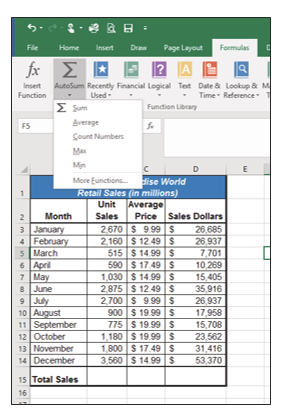
\includegraphics[width=\maxwidth{.95\linewidth}]{gfx/ch01_fig45}
			\caption{AutoSum Drop-Down List}
			\label{01:fig45}
		\end{figure}

		\item Click the \fmtButton{Sum} option from the \textit{AutoSum} drop-down menu. The first click will display a flashing marquee around the range. Tap \fmtKeystroke{Enter} or click the \fmtButton{Check Mark} next to the Formula bar to complete the function.
		\item Excel will provide a total for the values in the \textit{Unit Sales} column.
		\item It would not make sense to total the averages in \fmtLoc{Column C} so \fmtLoc{C15} will be left blank.
		\item Click in cell \fmtLoc{D15}. 
		\item Click \fmtButton{Formulas $ \Rightarrow $ Function Library $ \Rightarrow $ AutoSum $ \Rightarrow $ Down Arrow}. 
		\item Click the \fmtButton{Sum} option from the \textit{AutoSum} drop-down menu. The first click will display a flashing marquee around the range. Tap \fmtKeystroke{Enter} or click the \fmtButton{Check Mark} next to the Formula bar to complete the function (see Figure \ref{01:fig46}).
	\end{enumerate}
\end{enumbox}

\begin{figure}[H]
	\centering
	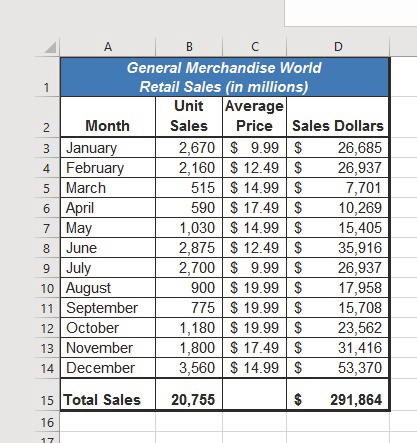
\includegraphics[width=\maxwidth{.95\linewidth}]{gfx/ch01_fig46}
	\caption{Totals Added to the Sheet1 Worksheet}
	\label{01:fig46}
\end{figure}

\begin{center}
	\begin{sklbox}{Skill Refresher}
		\textbf{AutoSum}
		\\
		\begin{itemize}
			\setlength{\itemsep}{0pt}
			\setlength{\parskip}{0pt}
			\setlength{\parsep}{0pt}
			
			\item Select a cell location below or to the right of a range of cells that contain numeric values.
			\item Click the \textit{Formulas} tab of the Ribbon.
			\item Click the down arrow below the \textit{AutoSum} button.
			\item Select a mathematical function from the list.
			
		\end{itemize}
	\end{sklbox}
\end{center}

\subsection{Moving, Renaming, Inserting, and Deleting Worksheets}

The default names for the worksheet tabs at the bottom of the workbook are numbered, starting with \textit{Sheet1}. However, the worksheet names can be changed to identify each worksheet's data. Additionally, the order in which the worksheet tabs appear can be changed. The following steps explain how to rename and move the worksheets in a workbook.

\begin{enumbox}
	\begin{enumerate}
		\item Double-click the \fmtWorksheet{Sheet1} worksheet tab at the bottom of the workbook (see Figure \ref{01:fig47}). 
		\item Type the name \fmtTyping{Sales by Month}, then tap  \fmtKeystroke{Enter}.
		\item Double click the \fmtWorksheet{Sheet2} worksheet tab at the bottom of the workbook.
		\item Type the name \fmtTyping{Unit Sales Rank}, then tap  \fmtKeystroke{Enter}.
	\end{enumerate}
\end{enumbox}

\begin{figure}[H]
	\centering
	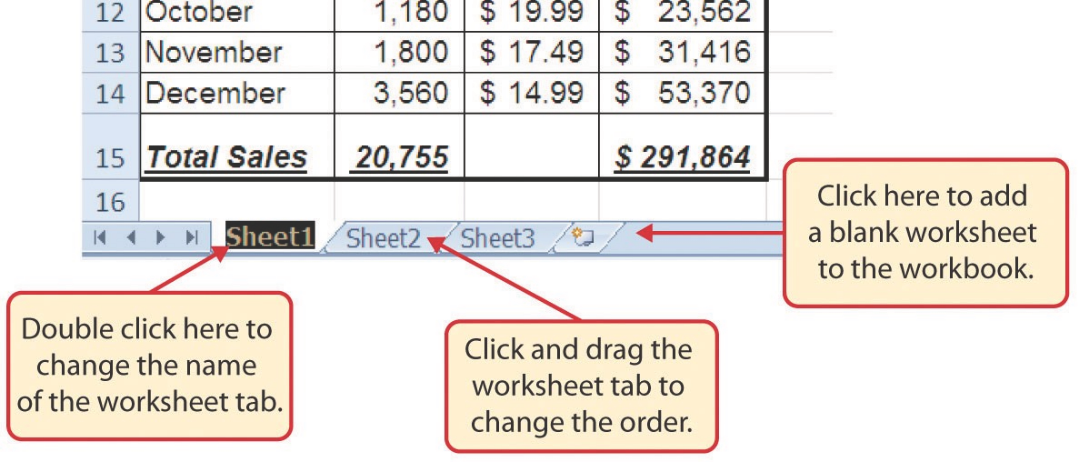
\includegraphics[width=\maxwidth{.95\linewidth}]{gfx/ch01_fig47}
	\caption{Renaming a Worksheet Tab}
	\label{01:fig47}
\end{figure}

\begin{enumbox}
	\begin{enumerate}
		\item Click and drag the \fmtWorksheet{Unit Sales Rank} worksheet tab to the \fmtWorksheet{Sales by Month} sheet's left. It will become the first worksheet in the workbook.
		\item Click the \fmtWorksheet{Sheet3} worksheet tab.
		\item Click \fmtButton{Home $ \Rightarrow $ Cells $ \Rightarrow $ Delete $ \Rightarrow $ Down Arrow $ \Rightarrow $ Delete Sheet} to remove the unneeded worksheet.
		\item If a warning box pops up, click the \fmtButton{Delete} button.
		\item Also, delete the \fmtWorksheet{Unit Sales Rank} worksheet since that worksheet is unnecessary. The workbook is left with just one worksheet, \fmtWorksheet{Sales by Month}.
		\item Save the changes to the workbook by clicking either \fmtButton{Quick Access Toolbar $ \Rightarrow $ Save} or \fmtButton{File $ \Rightarrow $ Save}.
	\end{enumerate}
\end{enumbox}
	
\begin{center}
	\begin{infobox}{Integrity Check}
		\textbf{Deleting Worksheets}
		\\
		\\
		Be very cautious when deleting worksheets that contain data. Once a worksheet is deleted, it is gone forever; the Undo command cannot return the sheet. \textit{Deleting a worksheet is permanent!}
	\end{infobox}
\end{center}

\begin{center}
	\begin{shtcutbox}{Keyboard Shortcuts}
		\textbf{Inserting New Worksheets}
		\\
		\begin{itemize}
			\setlength{\itemsep}{0pt}
			\setlength{\parskip}{0pt}
			\setlength{\parsep}{0pt}
			
			\item Press and hold \fmtKeystroke{Shift}, then tap \fmtKeystroke{F11}.
			
		\end{itemize}
	\end{shtcutbox}
\end{center}


Figure \ref{01:fig48} shows the final appearance of the \textit{CH1-GMW Sales} workbook.

\begin{figure}[H]
	\centering
	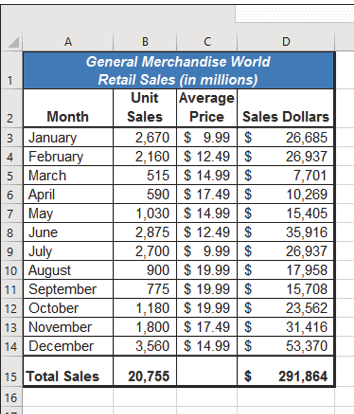
\includegraphics[width=\maxwidth{.95\linewidth}]{gfx/ch01_fig48}
	\caption{Final Appearance of the CH1-GMW Sales Workbook}
	\label{01:fig48}
\end{figure}

\begin{center}
	\begin{sklbox}{Skill Refresher}
		\textbf{Renaming Worksheets}
		\\
		\begin{itemize}
			\setlength{\itemsep}{0pt}
			\setlength{\parskip}{0pt}
			\setlength{\parsep}{0pt}
			
			\item Double click the worksheet tab.
			\item Type the new name.
			\item Tap \fmtKeystroke{Enter}.
		\end{itemize}

		\hfill \break
		\textbf{Moving Worksheets}
		\\
		\begin{itemize}
			\setlength{\itemsep}{0pt}
			\setlength{\parskip}{0pt}
			\setlength{\parsep}{0pt}
			
			\item Left-click the worksheet tab.
			\item Drag it to the desired position.
		\end{itemize}

		\hfill \break
		\textbf{Deleting Worksheets}
		\\
		\begin{itemize}
			\setlength{\itemsep}{0pt}
			\setlength{\parskip}{0pt}
			\setlength{\parsep}{0pt}
			
			\item Open the worksheet to be deleted.
			\item Click \textit{Home $ \Rightarrow $ Cells $ \Rightarrow $ Delete $ \Rightarrow $ Down Arrow $ \Rightarrow $ Delete Sheet}.
			\item Click \textit{Delete} on the warning box.
		\end{itemize}

	\end{sklbox}
\end{center}

\begin{center}
	\begin{infobox}{Best Practice}
		\textbf{Summary Worksheet}
		\\
		\\
		A good practice is to make the first worksheet in a workbook a summary. That sheet should include the workbook's purpose and a brief explanation for each worksheet. It should also include contact information for the originator so questions that may come up later can be clarified. The simple workbooks in this course will not include a summary sheet, but they would be included in more complex projects.
	\end{infobox}
\end{center}


\begin{center}
	\begin{tkwbox}{Key Take-Aways}
		\textbf{Save}
		\\
		\begin{itemize}
			\setlength{\itemsep}{0pt}
			\setlength{\parskip}{0pt}
			\setlength{\parsep}{0pt}
			
			\item Formatting skills are critical for creating worksheets that are easy to read and have a professional appearance.
			\item A series of hashtags (\#\#\#\#) in a cell location indicates that the column is too narrow to display the number entered.
			\item Using the Wrap Text command allows multi-word column headings to be stacked vertically in a cell location, reducing the need to expand column widths.
			\item Use the \textit{Merge \& Center} command to center the worksheet's title directly over the columns that contain data.
			\item Adding borders or lines will make the worksheet easier to read and helps to separate the data in each column and row.
			\item The Undo command will not bring back a worksheet that has been deleted.
			
			
		
		\end{itemize}
	\end{tkwbox}
\end{center}

\section{Printing}

\begin{center}
	\begin{objbox}{Learning Objectives}
		\begin{itemize}
			\setlength{\itemsep}{0pt}
			\setlength{\parskip}{0pt}
			\setlength{\parsep}{0pt}
			
			\item Use the \textit{Page Layout} tab to prepare a worksheet for printing.
			\item Add headers and footers to a printed worksheet.
			\item Explore how to print worksheets and workbooks.
		\end{itemize}
	\end{objbox}
\end{center}

Once a workbook is completed, selecting appropriate printing settings is a good practice. These settings are in the \textit{Page Layout} tab of the Ribbon and discussed in this chapter section.

\subsection{Page Setup}

The settings must be adjusted before the worksheets in a workbook can be printed. The following steps explain several of the commands in the \textit{Page Layout} tab of the Ribbon used to prepare a worksheet for printing.

\begin{enumbox}
	\begin{enumerate}
		\item Open the \fmtWorksheet{CH1-GMW Sales} workbook if it is not already open.
		\item Click \fmtButton{Page Layout $ \Rightarrow $ Page Setup $ \Rightarrow $ Margins} to open a drop-down list of options for setting the margins of the printed document. The \fmtButton{Normal}, \fmtButton{Wide}, and \fmtButton{Narrow} will quickly apply one of those standard margin settings and for this worksheet, click \fmtButton{Narrow}.
		\item Use \fmtButton{Page Layout $ \Rightarrow $ Page Setup $ \Rightarrow $ Margins $ \Rightarrow $ Custom Margins} to further adjust the margin settings
		\item On the \textit{Page Setup} dialog box, click the \fmtButton{Page} tab and select \fmtButton{Landscape}.
		\item Click the \textit{Margins} tab and locate the \fmtButton{Center on Page} section. Click the boxes to center the data horizontally and vertically on the worksheet (see Figure \ref{01:fig49}).
		\item Click \fmtButton{OK}.
	\end{enumerate}
\end{enumbox}

\begin{figure}[H]
	\centering
	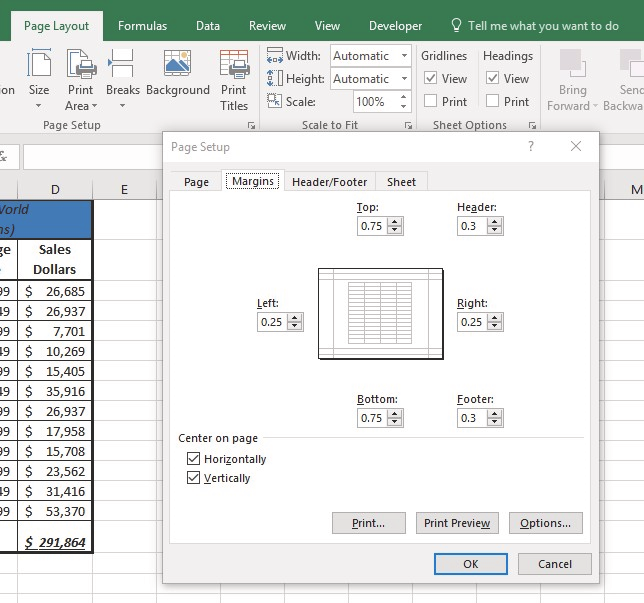
\includegraphics[width=\maxwidth{.95\linewidth}]{gfx/ch01_fig49}
	\caption{Page Layout Commands for Printing}
	\label{01:fig49}
\end{figure}

\begin{center}
	\begin{infobox}{Why?}
		\textbf{Use Print Settings}
		\\
		\\
		Because professionals often share Excel workbooks, selecting appropriate print settings in the \textit{Page Layout} tab is good even if there is no intent to print the worksheets. It can be highly frustrating to find that the necessary print settings are not set in a shared worksheet. 
	\end{infobox}
\end{center}

Table \ref{01:tab02} lists the various page layout settings and how they would be used.

\begin{table}[H]
	\rowcolors{1}{}{tablerow} % zebra striping background
	{\fontsize{8}{10} \selectfont %\small
		%\fontsize{8}{10} \selectfont %Replace small for special font size
		\begin{longtable}{L{0.75in}L{1.75in}L{1.75in}} %Left-aligned, Max width: 4.25in
			\textbf{Command} & \textbf{Purpose} & \textbf{Use} \endhead
			\hline
			Margins & Sets the top, bottom, right, and left margin space for the printed document & 1. Click the Page Layout tab of the Ribbon.\newline2. Click the Margin button.\newline3. Click one of the preset margin options or click Custom Margins.\\
			Orientation & Sets the orientation of the printed document to either portrait or landscape & 1. Click the Page Layout tab of the Ribbon.\newline2. Click the Orientation button.\newline3. Click one of the preset orientation options.\\
			Size & Sets the paper size for the printed document & 1. Click the Page Layout tab of the Ribbon.\newline2. Click the Size button.\newline3. Click one of the preset paper size options or click More Paper Sizes. \\
			Print Area & Prints only a specific area or range of cells on a worksheet & 1. Select the cells on a worksheet to be printed.\newline2. Click the Page Layout tab of the Ribbon.\newline3. Click the Print Area button.\newline4. Click the Set Print Area option from the drop-down list. \\
			Breaks & Manually set the page breaks on a worksheet & 1. Activate a cell on the worksheet where the page break should be placed. Breaks are created above and to the left of the activated cell.\newline2. Click the Page Layout tab of the Ribbon.\newline3. Click the Breaks button.\newline4. Click the Insert Page Break option from the drop-down list. \\
			Background & Adds a picture behind the cell locations in a worksheet & 1. Click the Page Layout tab of the Ribbon.\newline2. Click the Background button.\newline3. Select a picture stored on the local computer or network. \\
			Print Titles & Used when printing large data sets that are several pages long. This command will repeat the column headings at the top of each printed page. & 1. Click the Page Layout tab of the Ribbon.\newline2. Click the Print Titles button.\newline3. Click in the Rows to Repeat at Top input box in the Page Setup dialog box.\newline4. Click any cell in the row containing the worksheet's column headings.\newline5. Click the OK button at the bottom of the Page Setup dialog box. \\

			\rowcolor{captionwhite}
			\caption{Purpose and Use for Page Setup Commands}
			\label{01:tab02}
		\end{longtable}
	} % End small
\end{table}

\subsection{Headers and Footers}

Adding headers and footers to a printed document is standard practice. The header or footer could include the date, page number, company name, and other elements. The following steps explain adding headers and footers to the \textit{CH1-GMW Sales Data} workbook.

\begin{enumbox}
	\begin{enumerate}
		\item Click \fmtButton{Insert $ \Rightarrow $ Text $ \Rightarrow $ Header \& Footer}. 
	\end{enumerate}
\end{enumbox}

Note: A new tab containing header and footer controls is added to the ribbon. \fmtOldExcel{Excel 2016} names the tab \textit{Design} and \fmtNewExcel{Excel 365} names it \textit{Header \& Footer}. Besides the tab's name, the following instructions are the same for both versions of Excel. Inserting a header or footer will also open the \textit{Page Layout} view of the worksheet, making it easy to add elements like the date or page number. Figure \ref{01:fig50} shows the tab used to work with headers and footers.

\begin{figure}[H]
	\centering
	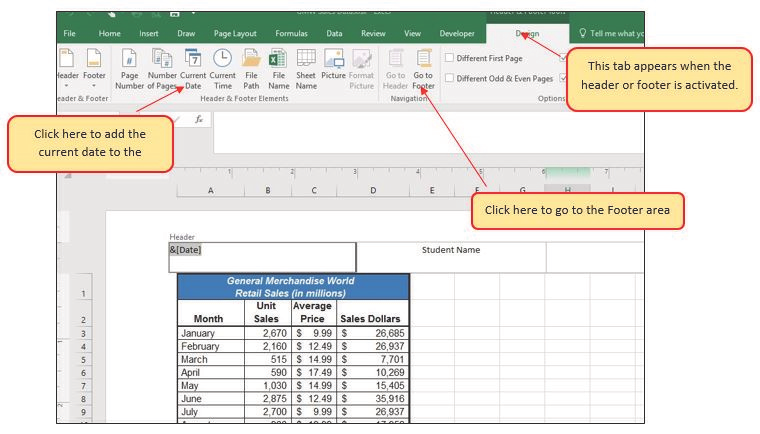
\includegraphics[width=\maxwidth{.95\linewidth}]{gfx/ch01_fig50}
	\caption{Tab for Creating Headers and Footers}
	\label{01:fig50}
\end{figure}

\begin{enumbox}
	\begin{enumerate}
		\item Type the author's name in the center section of the Header.
		\item Click in the left section of the Header (see Figure \ref{01:fig50}).
		\item Click \fmtButton{Design $ \Rightarrow $ Header \& Footer Elements $ \Rightarrow $ Current Date}. Note: the date will display as \textit{\&[Date]} until the workbook is printed or the normal view is restored.
		\item Click \fmtButton{Design $ \Rightarrow $ Navigation $ \Rightarrow $ Go To Footer}.
		\item Click in the right section of the footer.
		\item Click \fmtButton{Design $ \Rightarrow $ Header \& Footer $ \Rightarrow $ Page Number}. Note: the page number will display as \textit{\&[Page]} until the workbook is printed or the normal view is restored.
		\item Click any cell location outside the header or footer area.
		\item Click the \fmtButton{Normal} view button on the lower right side of the Status Bar (see Figure \ref{01:fig51}).
	\end{enumerate}
\end{enumbox}

\begin{figure}[H]
	\centering
	\includegraphics[width=\maxwidth{.95\linewidth}]{gfx/ch01_fig51}
	\caption{Worksheet in Page Layout View}
	\label{01:fig51}
\end{figure}

\subsection{Printing Worksheets and Workbooks}

Once the print settings have been adjusted and the headers and footers added, it is time to print the worksheet. The following steps explain printing the worksheet in the \textit{CH1-GMW Sales} workbook.

\begin{enumbox}
	\begin{enumerate}
		\item Click the \fmtButton{File} tab on the Ribbon.
		\item Click the \fmtButton{Print} option on the left side of the \textit{Backstage} view (see Figure \ref{01:fig52}). Notice that there is a preview of the printed worksheet on the right side of the \textit{Backstage} view.

		\begin{figure}[H]
			\centering
			\includegraphics[width=\maxwidth{.95\linewidth}]{gfx/ch01_fig52}
			\caption{Backstage View Print option}
			\label{01:fig52}
		\end{figure}

		\item Click the \fmtButton{Print Active Sheets} button in the \fmtButton{Print} section of the \textit{Backstage} view (see Figure \ref{01:fig52}).
		\item Click the \fmtButton{Print} button to print the active sheet.
		\item Click the \fmtButton{Home} tab of the Ribbon.
	%filesave CH1-GMW Sales Data
		\item Save the \fmtWorksheet{CH1-GMW Sales Data} workbook.
	%fileclose CH1-GMW Sales Data
	%filesolution CH1-GMW Sales Data Solution
		\item Compare the worksheet with the self-check answer key (\fmtWorksheet{CH1-GMW Sales Data Solution}) and then close and submit the \fmtWorksheet{CH1-GMW Sales Data} workbook as directed by the instructor.
	\end{enumerate}
\end{enumbox}
	
\begin{center}
	\begin{tkwbox}{Key Take-Aways}
		\textbf{Print}
		\\
		\begin{itemize}
			\setlength{\itemsep}{0pt}
			\setlength{\parskip}{0pt}
			\setlength{\parsep}{0pt}

			\item The commands in the Page Layout tab of the Ribbon are used to prepare a worksheet for printing.
			\item Headers and footers can be added to a worksheet to show essential information such as page number, date, and author's name.
			\item The \fmtButton{Print} commands are in the \fmtButton{File} tab of the Ribbon.
			
		\end{itemize}
	\end{tkwbox}
\end{center}

\section{Chapter Practice}

\subsection{Basic Monthly Budget for a Medical Office}

Creating and maintaining budgets are standard practices in many careers. Budgets play a critical role in helping a business or household control expenditures. A budget for a hypothetical medical office will be created in this exercise while reviewing the skills covered in this chapter.

\begin{enumbox}
	\begin{enumerate}
	%fileopen PR1-Data 
	%filesave PR1-Medical Office Budget
		\item Open the file named \fmtWorksheet{PR1-Data}, then save it as \fmtWorksheet{PR1-Medical Office Budget}.
		\item Activate all the cell locations in the \fmtWorksheet{Sheet1} worksheet by clicking the \fmtButton{Select All} button in the upper left corner of the worksheet (see Figure \ref{01:fig53}).

		\begin{figure}[H]
			\centering
			\includegraphics[width=\maxwidth{.95\linewidth}]{gfx/ch01_fig53}
			\caption{The Select All Button}
			\label{01:fig53}
		\end{figure}

		\item In the \fmtButton{Home} tab of the Ribbon, set the font style to Arial and the font size to $ 12 $ points. Then click any cell to deselect the worksheet.
		\item Double-click the divider between the tops of \fmtLoc{Column A} and \fmtLoc{Column B} to adjust \fmtLoc{Column A} so all entries are visible. 
		\item Click in \fmtLoc{B2} and enter \fmtTyping{Quarter 1}.
		\item Use \textit{AutoFill} to complete the headings in \fmtLoc{C2:E2}. Click in cell \fmtLoc{B2} and place the mouse pointer over the \textit{AutoFill Handle}. When the mouse pointer changes to a black plus sign, left-click and drag it to cell \fmtLoc{E2}.
		\item Click \fmtLoc{B2:E2} to select those cells. 
		\item Click \fmtButton{Home $ \Rightarrow $ Cells $ \Rightarrow $ Format $ \Rightarrow $ Column Width}. Set the column width to $ 11.57 $.
		\item Click \fmtLoc{A1} and enter \fmtTyping{Medical Office Budget}.
		\item Click on \fmtLoc{B1} and then click \fmtButton{Home $ \Rightarrow $ Cells $ \Rightarrow $ Insert $ \Rightarrow $ Insert Sheet Columns}.
		\item Click \fmtLoc{B2} and enter \fmtTyping{Budget Cost}.
		\item Adjust the width of \fmtLoc{Column B} to approximately $ 13.25 $ characters.
		\item Click and drag from \fmtLoc{A1} to \fmtLoc{F1} to select that range. 
		\item Click \fmtButton{Home $ \Rightarrow $ Alignment $ \Rightarrow $ Merge \& Center}.
		\item Make the following format adjustments to the merged range \fmtLoc{A1:F1}: bold; italics; change the font size to $ 14 $ points; change the cell fill color to Aqua-Accent $ 5 $-Darker $ 50 $\%, and change the font color to \textit{white}.
		\item Click \fmtLoc{A1}, then click \fmtButton{Home $ \Rightarrow $ Cells $ \Rightarrow $ Format $ \Rightarrow $ Row Height}. Set the height to $ 24.75 $.
		\item Make the following format adjustment to \fmtLoc{A2:F2}: bold; fill color to Tan-Background $ 2 $-Darker $ 10 $\%. Center the column titles so that they are horizontally centered in each cell.
		\item Select \fmtLoc{B2} and then click \fmtButton{Home $ \Rightarrow $ Alignment $ \Rightarrow $ Wrap Text}. 
		\item Copy cell \fmtLoc{C3} and paste the contents into \fmtLoc{D3:F3}.
		\item Click \fmtLoc{C6} and drag to \fmtLoc{C8} to select that range. Click \fmtButton{Home $ \Rightarrow $ Clipboard $ \Rightarrow $ Copy}.
		\item Click \fmtLoc{D6} and drag to \fmtLoc{F8} to select that range. Click \fmtButton{Home $ \Rightarrow $ Clipboard $ \Rightarrow $ Paste}.
		\item Click cell \fmtLoc{B3}. Click \fmtButton{Formulas $ \Rightarrow $ Function Library $ \Rightarrow $ AutoSum}. Click \fmtLoc{C3} and drag to \fmtLoc{F3} to select that range, then tap \fmtKeystroke{Enter} to complete the formula.
		\item Copy the formula in cell \fmtLoc{B3} and paste it into \fmtLoc{B4:B8}.
		\item Format \fmtLoc{B3:F8} with Accounting format and zero decimal places.
		\item Select \fmtLoc{A1:F8}.
		\item Click \fmtButton{Home $ \Rightarrow $ Font $ \Rightarrow $ Borders}. Select \fmtButton{All Borders}.
		\item Double-click the \fmtWorksheet{Sheet1} tab at the bottom of the worksheet, change its name to \fmtTyping{Budget}, then tap \fmtKeystroke{Enter}. 
		\item Delete all unused worksheets.
		\item Click \fmtButton{Page Layout $ \Rightarrow $ Page Setup $ \Rightarrow $ Orientation $ \Rightarrow $ Landscape}.
		\item Add a header to the \fmtWorksheet{Budget} worksheet that shows the current date in the upper left corner and the author's name in the center.
		\item Add a footer to the \fmtWorksheet{Budget} worksheet that shows the page number in the lower right corner. 
		\item Save the \fmtWorksheet{PR1-Medical Office Budget} workbook.
	%filesolution PR1-Medical Office Budget Solution
	%fileclose PR1-Medical Office Budget
		\item Compare the worksheet with the self-check answer key (\fmtWorksheet{PR1-Medical Office Budget Solution}) and then close and submit the \fmtWorksheet{PR1-Medical Office Budget} workbook as directed by the instructor.
	\end{enumerate}
\end{enumbox}
	
\section{Scored Assessment}

\subsection{Sales and Inventory Items}

Marketing professionals' essential activity is analyzing projected sales and inventory information, especially in retail environments. This exercise utilizes the skills this chapter covers to analyze sales and inventory data.

\begin{enumbox}
	\begin{enumerate}
	%fileopen SC1-Data
	%filesave SC1-Sales and Inventory
		\item Open the file named \fmtWorksheet{SC1-Data} and then save it as \fmtWorksheet{SC1-Sales and Inventory}
		\item In the \fmtWorksheet{Sheet1} worksheet, enter the word \fmtTyping{Totals} in cell \fmtLoc{C14}.
		\item Format all the cells in \fmtWorksheet{Sheet1} to Century font style and 12-point font size.
		\item Set the column width for \fmtLoc{Column A} through \fmtLoc{Column G} to $ 13.5 $.
		\item Edit the entry in cell \fmtLoc{B2} to read \fmtTyping{Item Number}.
		\item Use \textit{AutoFill} to fill the Item Numbers from \fmtLoc{B3} into \fmtLoc{B4:B13}. The item numbers should increase by one as they are filled through the range, so \fmtLoc{B13} is $ A1510 $.
		\item Copy the content of cell \fmtLoc{A3} and paste it into \fmtLoc{A4:A8}.
		\item Delete \fmtLoc{Column F}.
		\item Set \fmtLoc{A1:F2} to Bold.
		\item Set the alignment in \fmtLoc{A2:F2} to Wrap Text.
		\item Prepare \fmtLoc{A1:F1} for the title text by changing the fill color of the cells in \fmtLoc{A1:F1} to \textit{Red, Accent $ 2 $, Darker 25\%}.
		\item Make the following font changes to\fmtLoc{A1:F1}: set the font color to \textit{white}, add italics, and set the font size to $ 14 $.
		\item Merge and center the cells in \fmtLoc{A1:F1}.
		\item Enter the title for this worksheet in \fmtLoc{A1:F1}. The title should appear on two lines. The first line should read \fmtTyping{Status Report}, and the second line should read \fmtTyping{Sales and Inventory by Item}.
		\item Increase the height of \fmtLoc{Row 1} to make the entire title visible.
		\item Format the values in \fmtLoc{C3:C13} with dollar signs and two decimal places.
		\item Format the values in \fmtLoc{E3:F13} with comma style and zero decimal places.
		\item In cell \fmtLoc{E14}, use \fmtButton{AutoSum} to calculate the sum of the values in \fmtLoc{E3:E13}.
		\item In cell \fmtLoc{F14}, use \fmtButton{AutoSum} to calculate the sum of the values in \fmtLoc{F3:F13}.
		\item Apply \fmtButton{All Borders} to \fmtLoc{A1:F14}.
		\item Add a thick bottom border to \fmtLoc{A2:F2}; add a thick bottom border to \fmtLoc{A13:F13}.
		\item Add a thick outside border around the perimeter of \fmtLoc{A1:F14}.
		\item Insert a new blank worksheet in the workbook (\fmtWorksheet{Sheet4}).
		\item Delete \fmtWorksheet{Sheet3}.
		\item Move \fmtWorksheet{Sheet4} ahead of \fmtWorksheet{Sheet2} to make the worksheet order \fmtWorksheet{Sheet1}, \fmtWorksheet{Sheet4}, and \fmtWorksheet{Sheet2}.
		\item Rename the \fmtWorksheet{Sheet1} worksheet tab to \fmtTyping{Status Report}.
		\item Change the orientation of the \fmtWorksheet{Status Report} worksheet, so it prints landscape instead of portrait.
		\item Add a header to the \fmtWorksheet{Status Report} worksheet that shows the date in the upper left corner and the author's name in the center.
		\item Add a footer to the \fmtWorksheet{Status Report} worksheet that shows the page number in the lower right corner with the word \fmtTyping{Page} before the number.
		\item Center the worksheet both horizontally and vertically on the page.
	%filesave SC1-Sales and Inventory
	%fileclose SC1-Sales and Inventory
		\item Save and close the \fmtWorksheet{SC1-Sales and Inventory} workbook.
		\item Submit the \fmtWorksheet{SC1-Sales and Inventory} workbook as directed by the instructor.
	\end{enumerate}
\end{enumbox}